\documentclass[a4paper,twoside,7pt]{book}

\usepackage{latexsym}%symbole
\usepackage[empty]{fullpage}
\usepackage{titlesec}%alternatywne sekcje tytułowe
\usepackage{marvosym}%wiecej symboli
\usepackage[usenames,dvipsnames]{color}
\usepackage{verbatim}%wyświetlanie kodu
\usepackage{enumitem}%zmienianie layoutu
\usepackage[hidelinks]{hyperref}%?!?!?!
\usepackage{fancyhdr}%heders and footers
\usepackage[english]{babel}%znaki lokalne?
\usepackage{tabularx}% tabeli 
\usepackage{multicol}% wiele column
\usepackage{minted}% syntax hilighting
\input{glyphtounicode}

\usepackage{baskervillef}
\usepackage[T1]{fontenc}
%flow chatry
\usepackage{tikz}
\usetikzlibrary{shapes.geometric, arrows}
\usepackage{amssymb}
\usepackage{float}
\usepackage{pgf}

\pagestyle{fancy}
\fancyhf{} 
\fancyfoot[OR]{\thepage}
\fancyfoot[EL]{\thepage}
\setlength{\footskip}{5pt}
\renewcommand{\headrulewidth}{0pt}
\renewcommand{\footrulewidth}{0pt}

\usepackage[left=0.5in,right=0.5in,top=0.5in,bottom=0.5in,inner=2.6cm]{geometry}

\urlstyle{same}

%\raggedbottom
\raggedright
\setlength{\tabcolsep}{0in}

\titleformat{\section}{
  \it\vspace{3pt}
}{}{0em}{}[\color{black}\titlerule\vspace{-5pt}]

\pdfgentounicode=1
%flowchatrts shapes

\definecolor{1}{RGB}{128, 147, 241}
\definecolor{2}{RGB}{114, 221, 247}
\definecolor{3}{RGB}{179, 136, 235}
\definecolor{4}{RGB}{247, 174, 248}

\tikzstyle{startstop} = [ellipse, rounded corners, minimum width=2cm, minimum height=1cm,text centered, draw=black,thick,fill=4]
\tikzstyle{io} = [trapezium,trapezium stretches=true,trapezium left angle=70,trapezium right angle=110,thick,minimum width=1cm,minimum height=0.85cm, text centered, draw=black,fill=1]
\tikzstyle{process} = [rectangle,minimum width=1cm,minimum height=0.85cm,text centered,draw=black,thick,fill=2]
\tikzstyle{decision} = [diamond,minimum width=1cm, minimum height=1cm, text centered, draw=black, fill=3,thick]
\tikzstyle{arrow} = [thick,->,>=stealth]
\tikzstyle{none} = [coordinate]
\tikzstyle{con} = [thick]

\begin{document}
\raggedcolumns
\begin{center}
    \begin{multicols}{2}
    \begin{flushleft}
    \large{Tymon Łazowy 3D nr.09} \\
    \end{flushleft}
    
    \begin{flushright}
    \large{29.09.2023}\\
    \end{flushright}
    \end{multicols}
    {\LARGE Sprawozdanie z informatyki nr 2} \\ \vspace{0pt}
\end{center}

\section{Treść zadanie}
\begin{center}
\large{Programownie część Druga}\\

\begin{itemize}[ label={}]
    \normalsize{\item{
    {2.1 - Program przeliczający waluty}{} \\
    {2.2 - Program obliczający pola i obwody 4 figur geometrycznych foremnych}{} \\
    {2.3 - Program sprawdzający ile jest cyfr w liczbie całkowitej z przedziału <0,miliard> \\
    {2.4 - Liczby podzielne z przedziału}{} \\
    {2.5 - Średnia arytmetyczna z n liczb podanych przez użytkownika}{} \\
    {2.6 - Wyświetlenie i zliczenie wszystkich naturalnych liczb trzycyfrowych w których suma
cyfr wynosi n}{} \\
    {2.7 - Przerób program 2.6 tak, aby działał w pętli}{} \\
    {2.8 - Średnia arytmetyczna z n liczb dwucyfrowych, dodatnich podanych przez użytkownika}{} \\
    {2.9 - Program obliczający NWD i NWW 2 liczb a i b}{} \\
    {2.10 - Tabliczka mnożenia od-do}{} \\
    {2.11 - Szukanie minimalnej liczby z ciągu liczb dwucyfrowych podawanych przez użytkownika}{}\\
    {2.12 - Program obliczający NWD z 2 liczb(odejmowanie)}{}\\
    {2.13 - Obliczanie n! dla liczby naturalnej n>=0 – algorytm iteracyjny}{}\\
    {2.14 - Obliczanie wartości n-tego wyrazu ciągu Fibonacciego (n>=1) – algorytm iteracyjny}{}\\
    {2.15 - Sprawdzanie czy liczba n (n>0) jest liczbą pierwszą}{}\\
    {2.16 -  Suma cyfr liczby całkowitej n (n>0)}{}\\
}}}
\end{itemize}

\end{center}
%---------------------PROPONOWANE ROZWIĄZANIA-------------

\section{Proponowane rozwiązania}
\subsection*{2.1}
%----------------2.1------------------
\subsection*{dis()}
\begin{multicols}{2}
  \begin{flushleft}
\renewcommand{\thefigure}{1.0}
\begin{figure}[H]
    \centering  
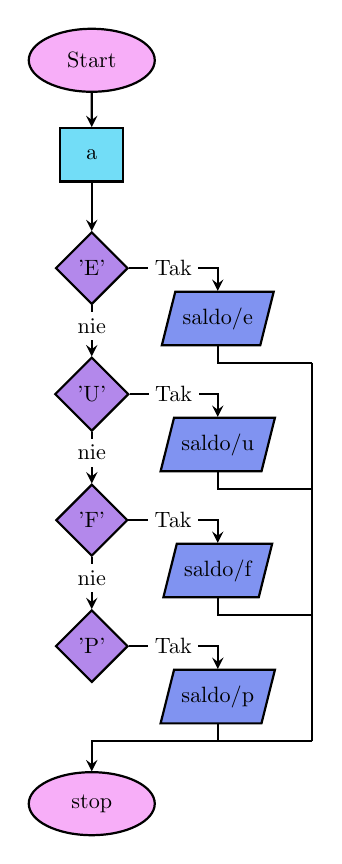
\begin{tikzpicture}[scale=0.8,transform shape,node distance=1.5cm]

\node (start) [startstop] {Start};
\node (s1) [process, below of=start] {a};

\node (c1) [decision, below of=s1,yshift=-0.3cm] {'E'};
\node (out1) [io, right of=c1, xshift=0.5cm, yshift=-0.8cm] {saldo/e};

\node (c2) [decision, below of=c1,yshift=-0.5cm] {'U'};
\node (out2) [io, right of=c2, xshift=0.5cm, yshift=-0.8cm] {saldo/u};

\node (c3) [decision, below of=c2,yshift=-0.5cm] {'F'};
\node (out3) [io, right of=c3, xshift=0.5cm, yshift=-0.8cm] {saldo/f};

\node (c4) [decision, below of=c3,yshift=-0.5cm] {'P'};
\node (out4) [io, right of=c4, xshift=0.5cm, yshift=-0.8cm] {saldo/p};

\node (e1)[coordinate,below of=c1,xshift=3.5cm]{};
\node (e2)[coordinate,below of=c2,xshift=3.5cm]{};
\node (e3)[coordinate,below of=c3,xshift=3.5cm]{};
\node (e4)[coordinate,below of=c4,xshift=3.5cm]{};

\node (stop) [startstop, below of =c4,yshift=-1cm]{stop};

\draw [arrow] (start) -- (s1);

\draw [arrow] (s1) -- (c1);
\draw [arrow] (c1) -- (c2)node[pos=0.4,fill=white,inner sep=3]{nie};
\draw [arrow] (c2) -- (c3)node[pos=0.4,fill=white,inner sep=3]{nie};
\draw [arrow] (c3) -- (c4)node[pos=0.4,fill=white,inner sep=3]{nie};
\draw [arrow] (c1) -| (out1)node[pos=0.25,fill=white,inner sep=3]{Tak};
\draw [arrow] (c2) -| (out2)node[pos=0.25,fill=white,inner sep=3]{Tak};
\draw [arrow] (c3) -| (out3)node[pos=0.25,fill=white,inner sep=3]{Tak};
\draw [arrow] (c4) -| (out4)node[pos=0.25,fill=white,inner sep=3]{Tak};

\draw [thick] (out1) |- (e1);
\draw [thick] (out2) |- (e2);
\draw [thick] (out3) |- (e3);
\draw [thick] (out4) |- (e4);

\draw [thick] (e1) |- (e4);

\draw [arrow] (e4) -| (stop);

\end{tikzpicture}
    \caption{funcion dis() flowchart}
    \label{flow1.2}
\end{figure}

    \end{flushleft}
D: \\
Saldo, kwota pieniedzy $\in$ $\mathbb{R}$\\
c, waluta $\in$ \{u,f,p,e\}\\
W: strumień, saldo w innych walutach $\in$ $\mathbb{R}$
    \begin{flushright}
    \renewcommand{\thefigure}{1.0}
\begin{figure}[H]
    \centering  
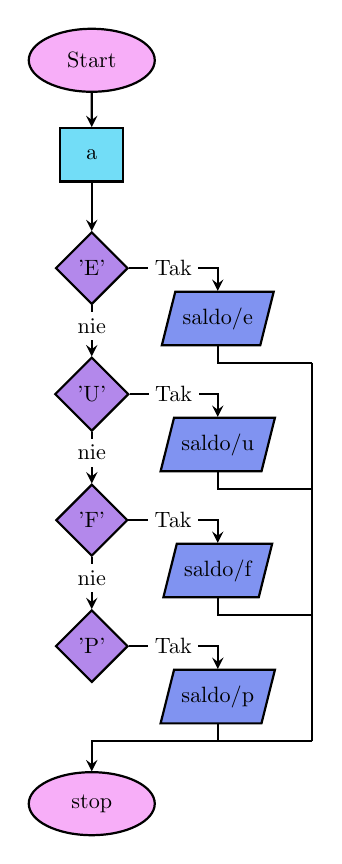
\begin{tikzpicture}[scale=0.8,transform shape,node distance=1.5cm]

\node (start) [startstop] {Start};
\node (s1) [process, below of=start] {a};

\node (c1) [decision, below of=s1,yshift=-0.3cm] {'E'};
\node (out1) [io, right of=c1, xshift=0.5cm, yshift=-0.8cm] {saldo/e};

\node (c2) [decision, below of=c1,yshift=-0.5cm] {'U'};
\node (out2) [io, right of=c2, xshift=0.5cm, yshift=-0.8cm] {saldo/u};

\node (c3) [decision, below of=c2,yshift=-0.5cm] {'F'};
\node (out3) [io, right of=c3, xshift=0.5cm, yshift=-0.8cm] {saldo/f};

\node (c4) [decision, below of=c3,yshift=-0.5cm] {'P'};
\node (out4) [io, right of=c4, xshift=0.5cm, yshift=-0.8cm] {saldo/p};

\node (e1)[coordinate,below of=c1,xshift=3.5cm]{};
\node (e2)[coordinate,below of=c2,xshift=3.5cm]{};
\node (e3)[coordinate,below of=c3,xshift=3.5cm]{};
\node (e4)[coordinate,below of=c4,xshift=3.5cm]{};

\node (stop) [startstop, below of =c4,yshift=-1cm]{stop};

\draw [arrow] (start) -- (s1);

\draw [arrow] (s1) -- (c1);
\draw [arrow] (c1) -- (c2)node[pos=0.4,fill=white,inner sep=3]{nie};
\draw [arrow] (c2) -- (c3)node[pos=0.4,fill=white,inner sep=3]{nie};
\draw [arrow] (c3) -- (c4)node[pos=0.4,fill=white,inner sep=3]{nie};
\draw [arrow] (c1) -| (out1)node[pos=0.25,fill=white,inner sep=3]{Tak};
\draw [arrow] (c2) -| (out2)node[pos=0.25,fill=white,inner sep=3]{Tak};
\draw [arrow] (c3) -| (out3)node[pos=0.25,fill=white,inner sep=3]{Tak};
\draw [arrow] (c4) -| (out4)node[pos=0.25,fill=white,inner sep=3]{Tak};

\draw [thick] (out1) |- (e1);
\draw [thick] (out2) |- (e2);
\draw [thick] (out3) |- (e3);
\draw [thick] (out4) |- (e4);

\draw [thick] (e1) |- (e4);

\draw [arrow] (e4) -| (stop);

\end{tikzpicture}
    \caption{funcion dis() flowchart}
    \label{flow1.2}
\end{figure}

    \end{flushright}
\end{multicols}
\newpage
\subsection*{Main}
\begin{multicols}{2}
  \begin{flushleft}
\renewcommand{\thefigure}{1}
\begin{figure}[H]
  \centering  
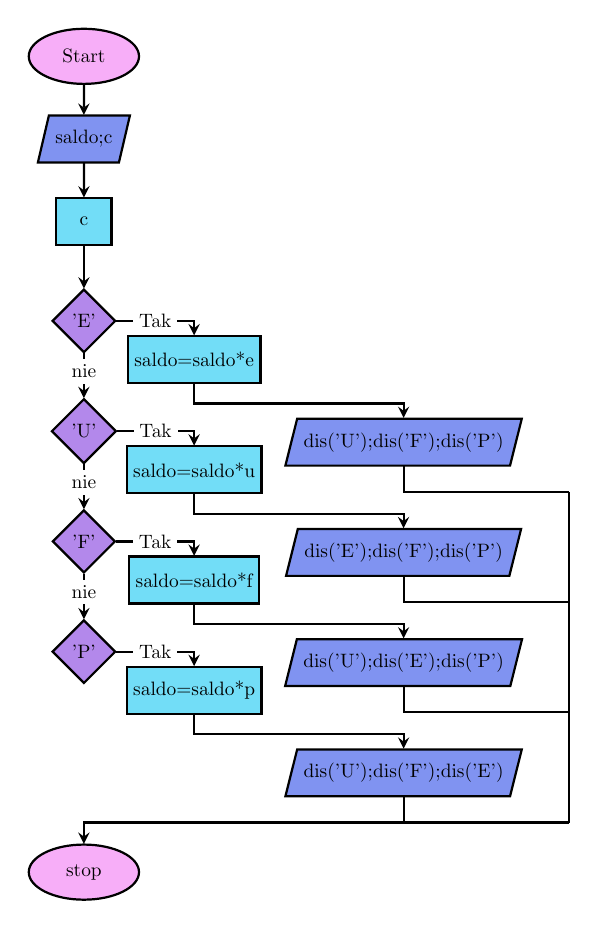
\begin{tikzpicture}[scale=0.7,transform shape,node distance=1.5cm]

\node (start) [startstop] {Start};
\node (in1) [io, below of=start] {saldo;c};
\node (s1) [process, below of=in1] {c};

\node (c1) [decision, below of=s1,yshift=-0.3cm] {'E'};
\node (p1) [process, below of=c1, xshift=2cm,yshift=0.8cm] {saldo=saldo*e};
\node (out1) [io, right of=p1, xshift=2.3cm, yshift=-1.5cm] {dis('U');dis('F');dis('P')};

\node (c2) [decision, below of=c1,yshift=-0.5cm] {'U'};
\node (p2) [process, below of=c2, xshift=2cm,yshift=0.8cm] {saldo=saldo*u};
\node (out2) [io, right of=p2, xshift=2.3cm, yshift=-1.5cm] {dis('E');dis('F');dis('P')};

\node (c3) [decision, below of=c2,yshift=-0.5cm] {'F'};
\node (p3) [process, below of=c3, xshift=2cm,yshift=0.8cm] {saldo=saldo*f};
\node (out3) [io, right of=p3, xshift=2.3cm, yshift=-1.5cm] {dis('U');dis('E');dis('P')};

\node (c4) [decision, below of=c3,yshift=-0.5cm] {'P'};
\node (p4) [process, below of=c4, xshift=2cm,yshift=0.8cm] {saldo=saldo*p};
\node (out4) [io, right of=p4, xshift=2.3cm, yshift=-1.5cm] {dis('U');dis('F');dis('E')};

\node (e1)[coordinate,below of=c1,xshift=4.5cm]{};
\node (e2)[coordinate,below of=c2,xshift=4.5cm]{};
\node (e3)[coordinate,below of=c3,xshift=4.5cm]{};
\node (e4)[coordinate,below of=c4,xshift=4.5cm]{};
\node (e5)[coordinate,below of=out1,yshift=0.6cm,xshift=3cm]{};
\node (e6)[coordinate,below of=out2,yshift=0.6cm,xshift=3cm]{};
\node (e7)[coordinate,below of=out3,yshift=0.6cm,xshift=3cm]{};
\node (e8)[coordinate,below of=out4,yshift=0.6cm,xshift=3cm]{};

\node (stop) [startstop, below of =c4,yshift=-2.5cm]{stop};

\draw [arrow] (start) -- (in1);
\draw [arrow] (in1) -- (s1);
\draw [arrow] (s1) -- (c1);
\draw [arrow] (c1) -- (c2)node[pos=0.4,fill=white,inner sep=3]{nie};
\draw [arrow] (c2) -- (c3)node[pos=0.4,fill=white,inner sep=3]{nie};
\draw [arrow] (c3) -- (c4)node[pos=0.4,fill=white,inner sep=3]{nie};
\draw [arrow] (c1) -| (p1)node[pos=0.25,fill=white,inner sep=3]{Tak};
\draw [arrow] (c2) -| (p2)node[pos=0.25,fill=white,inner sep=3]{Tak};
\draw [arrow] (c3) -| (p3)node[pos=0.25,fill=white,inner sep=3]{Tak};
\draw [arrow] (c4) -| (p4)node[pos=0.25,fill=white,inner sep=3]{Tak};

\draw [thick] (p1) |- (e1);
\draw [thick] (p2) |- (e2);
\draw [thick] (p3) |- (e3);
\draw [thick] (p4) |- (e4);

\draw [arrow] (e1) -| (out1);
\draw [arrow] (e2) -| (out2);
\draw [arrow] (e3) -| (out3);
\draw [arrow] (e4) -| (out4);

\draw [thick] (out1) |- (e5);
\draw [thick] (out2) |- (e6);
\draw [thick] (out3) |- (e7);
\draw [thick] (out4) |- (e8);

\draw [thick] (e5) |- (e8);


\draw [arrow] (e8) -| (stop);


\end{tikzpicture}
    \caption{2.1 flowchart}
    \label{flow1}
\end{figure}

    \end{flushleft}
D: \\
Saldo, kwota pieniedzy $\in$ $\mathbb{R}$\\
c, waluta $\in$ \{u,f,p,e\}\\
W: strumień, saldo w innych walutach $\in$ $\mathbb{R}$
    \begin{flushright}
    \renewcommand{\thefigure}{1}
\begin{figure}[H]
  \centering  
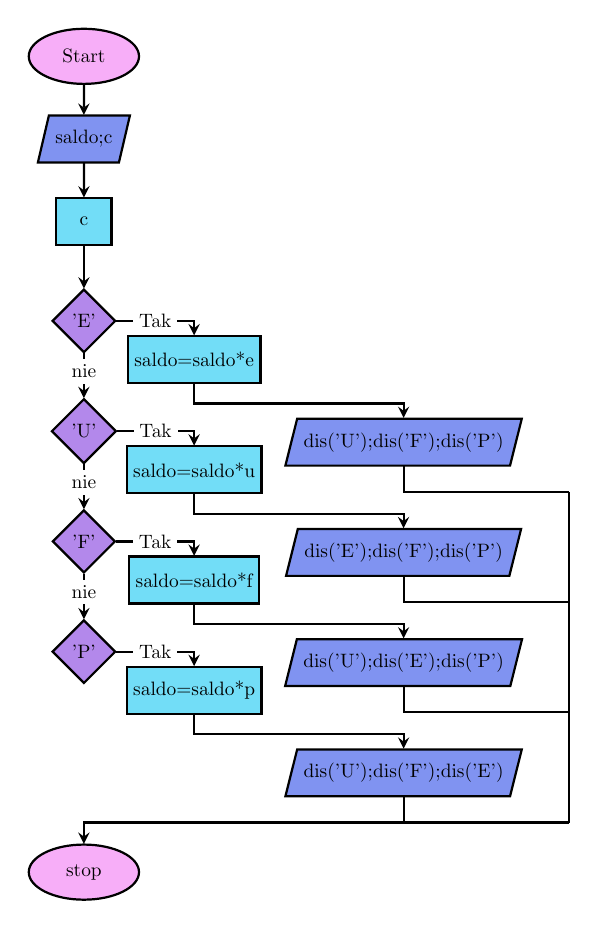
\begin{tikzpicture}[scale=0.7,transform shape,node distance=1.5cm]

\node (start) [startstop] {Start};
\node (in1) [io, below of=start] {saldo;c};
\node (s1) [process, below of=in1] {c};

\node (c1) [decision, below of=s1,yshift=-0.3cm] {'E'};
\node (p1) [process, below of=c1, xshift=2cm,yshift=0.8cm] {saldo=saldo*e};
\node (out1) [io, right of=p1, xshift=2.3cm, yshift=-1.5cm] {dis('U');dis('F');dis('P')};

\node (c2) [decision, below of=c1,yshift=-0.5cm] {'U'};
\node (p2) [process, below of=c2, xshift=2cm,yshift=0.8cm] {saldo=saldo*u};
\node (out2) [io, right of=p2, xshift=2.3cm, yshift=-1.5cm] {dis('E');dis('F');dis('P')};

\node (c3) [decision, below of=c2,yshift=-0.5cm] {'F'};
\node (p3) [process, below of=c3, xshift=2cm,yshift=0.8cm] {saldo=saldo*f};
\node (out3) [io, right of=p3, xshift=2.3cm, yshift=-1.5cm] {dis('U');dis('E');dis('P')};

\node (c4) [decision, below of=c3,yshift=-0.5cm] {'P'};
\node (p4) [process, below of=c4, xshift=2cm,yshift=0.8cm] {saldo=saldo*p};
\node (out4) [io, right of=p4, xshift=2.3cm, yshift=-1.5cm] {dis('U');dis('F');dis('E')};

\node (e1)[coordinate,below of=c1,xshift=4.5cm]{};
\node (e2)[coordinate,below of=c2,xshift=4.5cm]{};
\node (e3)[coordinate,below of=c3,xshift=4.5cm]{};
\node (e4)[coordinate,below of=c4,xshift=4.5cm]{};
\node (e5)[coordinate,below of=out1,yshift=0.6cm,xshift=3cm]{};
\node (e6)[coordinate,below of=out2,yshift=0.6cm,xshift=3cm]{};
\node (e7)[coordinate,below of=out3,yshift=0.6cm,xshift=3cm]{};
\node (e8)[coordinate,below of=out4,yshift=0.6cm,xshift=3cm]{};

\node (stop) [startstop, below of =c4,yshift=-2.5cm]{stop};

\draw [arrow] (start) -- (in1);
\draw [arrow] (in1) -- (s1);
\draw [arrow] (s1) -- (c1);
\draw [arrow] (c1) -- (c2)node[pos=0.4,fill=white,inner sep=3]{nie};
\draw [arrow] (c2) -- (c3)node[pos=0.4,fill=white,inner sep=3]{nie};
\draw [arrow] (c3) -- (c4)node[pos=0.4,fill=white,inner sep=3]{nie};
\draw [arrow] (c1) -| (p1)node[pos=0.25,fill=white,inner sep=3]{Tak};
\draw [arrow] (c2) -| (p2)node[pos=0.25,fill=white,inner sep=3]{Tak};
\draw [arrow] (c3) -| (p3)node[pos=0.25,fill=white,inner sep=3]{Tak};
\draw [arrow] (c4) -| (p4)node[pos=0.25,fill=white,inner sep=3]{Tak};

\draw [thick] (p1) |- (e1);
\draw [thick] (p2) |- (e2);
\draw [thick] (p3) |- (e3);
\draw [thick] (p4) |- (e4);

\draw [arrow] (e1) -| (out1);
\draw [arrow] (e2) -| (out2);
\draw [arrow] (e3) -| (out3);
\draw [arrow] (e4) -| (out4);

\draw [thick] (out1) |- (e5);
\draw [thick] (out2) |- (e6);
\draw [thick] (out3) |- (e7);
\draw [thick] (out4) |- (e8);

\draw [thick] (e5) |- (e8);


\draw [arrow] (e8) -| (stop);


\end{tikzpicture}
    \caption{2.1 flowchart}
    \label{flow1}
\end{figure}

    \end{flushright}
\end{multicols}

\subsection*{2.2}
%----------------2.2------------------
\begin{multicols}{2}
  \begin{flushleft}
\renewcommand{\thefigure}{2}
\begin{figure}[H]
    \centering  
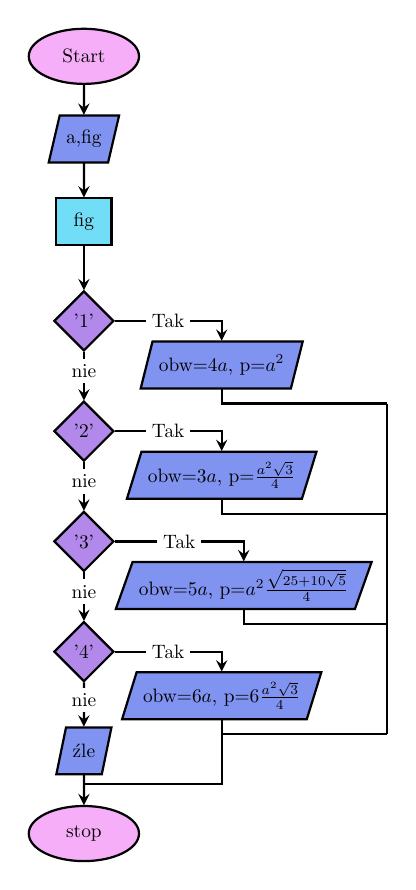
\begin{tikzpicture}[scale=0.7,transform shape,node distance=1.5cm]

\node (start) [startstop] {Start};
\node (in1) [io, below of=start] {a,fig};
\node (s1) [process, below of=in1] {fig};

\node (c1) [decision, below of=s1,yshift=-0.3cm] {'1'};
\node (out1) [io, right of=c1, xshift=1cm, yshift=-0.8cm] {obw=$4a$, p=$a^2$};

\node (c2) [decision, below of=c1,yshift=-0.5cm] {'2'};
\node (out2) [io, right of=c2, xshift=1cm, yshift=-0.8cm] {obw=$3a$, p=$\frac{a^2\sqrt{3}}{4}$};

\node (c3) [decision, below of=c2,yshift=-0.5cm] {'3'};
\node (out3) [io, right of=c3, xshift=1.4cm, yshift=-0.8cm] {obw=$5a$, p=$a^2\frac{\sqrt{25+10\sqrt{5}}}{4}$};

\node (c4) [decision, below of=c3,yshift=-0.5cm] {'4'};
\node (out4) [io, right of=c4, xshift=1cm, yshift=-0.8cm] {obw=$6a$, p=$6\frac{a^2\sqrt{3}}{4}$};

\node (c5) [io, below of=c4, yshift=-0.3cm] {źle};

\node (e1)[coordinate,below of=c1,xshift=5.5cm]{};
\node (e2)[coordinate,below of=c2,xshift=5.5cm]{};
\node (e3)[coordinate,below of=c3,xshift=5.5cm]{};
\node (e4)[coordinate,below of=c4,xshift=5.5cm]{};
\node (e5)[coordinate,below of=c5,yshift=0.9cm]{};

\node (stop) [startstop, below of =c5,yshift=0cm]{stop};

\draw [arrow] (start) -- (in1);
\draw [arrow] (in1) -- (s1);
\draw [arrow] (s1) -- (c1);

\draw [arrow] (c1) -- (c2)node[pos=0.4,fill=white,inner sep=3]{nie};
\draw [arrow] (c2) -- (c3)node[pos=0.4,fill=white,inner sep=3]{nie};
\draw [arrow] (c3) -- (c4)node[pos=0.4,fill=white,inner sep=3]{nie};
\draw [arrow] (c4) -- (c5)node[pos=0.4,fill=white,inner sep=3]{nie};
\draw [arrow] (c1) -| (out1)node[pos=0.25,fill=white,inner sep=3]{Tak};
\draw [arrow] (c2) -| (out2)node[pos=0.25,fill=white,inner sep=3]{Tak};
\draw [arrow] (c3) -| (out3)node[pos=0.25,fill=white,inner sep=3]{Tak};
\draw [arrow] (c4) -| (out4)node[pos=0.25,fill=white,inner sep=3]{Tak};

\draw [thick] (out1) |- (e1);
\draw [thick] (out2) |- (e2);
\draw [thick] (out3) |- (e3);
\draw [thick] (out4) |- (e4);

\draw [thick] (e1) |- (e4);
\draw [thick] (out4) |- (e5);

\draw [arrow] (c5) -- (stop);

\end{tikzpicture}
    \caption{2.2 flowchart}
    \label{flow2}
\end{figure}

    \end{flushleft}
D: a, długość boku >= 0 $\in$ $\mathbb{R}$\\
fig, typ figury $\in$ \{1;2;3;4\}\\
W: p, pole >= 0 $\in$ $\mathbb{R}$\\
obw, obwód >=0 $\in$ $\mathbb{R}$
    \begin{flushright}
    \renewcommand{\thefigure}{2}
\begin{figure}[H]
    \centering  
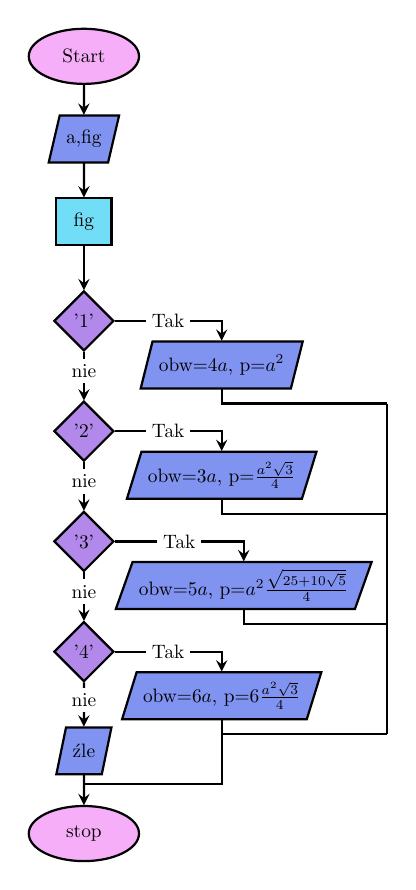
\begin{tikzpicture}[scale=0.7,transform shape,node distance=1.5cm]

\node (start) [startstop] {Start};
\node (in1) [io, below of=start] {a,fig};
\node (s1) [process, below of=in1] {fig};

\node (c1) [decision, below of=s1,yshift=-0.3cm] {'1'};
\node (out1) [io, right of=c1, xshift=1cm, yshift=-0.8cm] {obw=$4a$, p=$a^2$};

\node (c2) [decision, below of=c1,yshift=-0.5cm] {'2'};
\node (out2) [io, right of=c2, xshift=1cm, yshift=-0.8cm] {obw=$3a$, p=$\frac{a^2\sqrt{3}}{4}$};

\node (c3) [decision, below of=c2,yshift=-0.5cm] {'3'};
\node (out3) [io, right of=c3, xshift=1.4cm, yshift=-0.8cm] {obw=$5a$, p=$a^2\frac{\sqrt{25+10\sqrt{5}}}{4}$};

\node (c4) [decision, below of=c3,yshift=-0.5cm] {'4'};
\node (out4) [io, right of=c4, xshift=1cm, yshift=-0.8cm] {obw=$6a$, p=$6\frac{a^2\sqrt{3}}{4}$};

\node (c5) [io, below of=c4, yshift=-0.3cm] {źle};

\node (e1)[coordinate,below of=c1,xshift=5.5cm]{};
\node (e2)[coordinate,below of=c2,xshift=5.5cm]{};
\node (e3)[coordinate,below of=c3,xshift=5.5cm]{};
\node (e4)[coordinate,below of=c4,xshift=5.5cm]{};
\node (e5)[coordinate,below of=c5,yshift=0.9cm]{};

\node (stop) [startstop, below of =c5,yshift=0cm]{stop};

\draw [arrow] (start) -- (in1);
\draw [arrow] (in1) -- (s1);
\draw [arrow] (s1) -- (c1);

\draw [arrow] (c1) -- (c2)node[pos=0.4,fill=white,inner sep=3]{nie};
\draw [arrow] (c2) -- (c3)node[pos=0.4,fill=white,inner sep=3]{nie};
\draw [arrow] (c3) -- (c4)node[pos=0.4,fill=white,inner sep=3]{nie};
\draw [arrow] (c4) -- (c5)node[pos=0.4,fill=white,inner sep=3]{nie};
\draw [arrow] (c1) -| (out1)node[pos=0.25,fill=white,inner sep=3]{Tak};
\draw [arrow] (c2) -| (out2)node[pos=0.25,fill=white,inner sep=3]{Tak};
\draw [arrow] (c3) -| (out3)node[pos=0.25,fill=white,inner sep=3]{Tak};
\draw [arrow] (c4) -| (out4)node[pos=0.25,fill=white,inner sep=3]{Tak};

\draw [thick] (out1) |- (e1);
\draw [thick] (out2) |- (e2);
\draw [thick] (out3) |- (e3);
\draw [thick] (out4) |- (e4);

\draw [thick] (e1) |- (e4);
\draw [thick] (out4) |- (e5);

\draw [arrow] (c5) -- (stop);

\end{tikzpicture}
    \caption{2.2 flowchart}
    \label{flow2}
\end{figure}

    \end{flushright}    
\end{multicols}
\newpage

\subsection*{2.3}
%----------------2.3------------------
\begin{multicols}{2}
  \begin{flushleft}
\renewcommand{\thefigure}{3}
\begin{figure}[H]
    \centering 
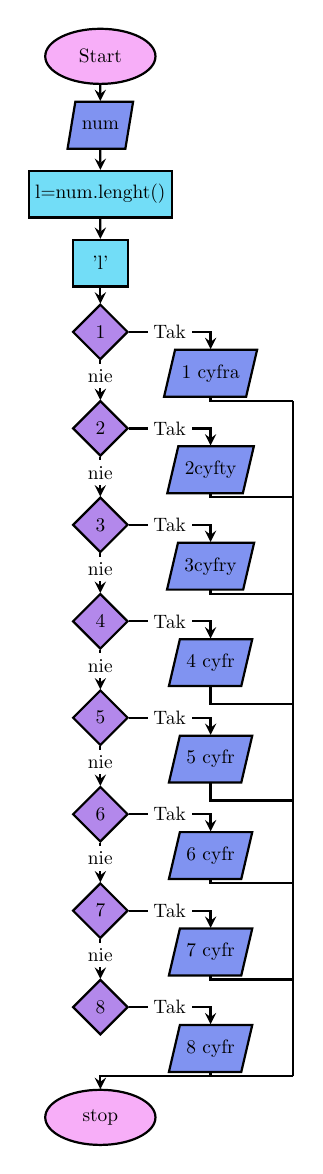
\begin{tikzpicture}[scale=0.7,transform shape]
		\node [style=startstop] (0) at (0, 0) {Start};
		\node [style=io] (1) at (0, -1.25) {num};
		\node [style=process] (3) at (0, -3.75) {'l'};
		\node [style=decision] (4) at (0, -5) {1};
		\node [style=decision] (5) at (0, -6.75) {2};
		\node [style=decision] (6) at (0, -8.5) {3};
		\node [style=decision] (7) at (0, -10.25) {4};
		\node [style=process] (8) at (0, -2.5) {l=num.lenght()};
		\node [style=decision] (9) at (0, -12) {5};
		\node [style=decision] (10) at (0, -13.75) {6};
		\node [style=decision] (11) at (0, -15.5) {7};
		\node [style=decision] (12) at (0, -17.25) {8};
		\node [style=io] (14) at (2, -5.75) {1 cyfra};
		\node [style=io] (15) at (2, -7.5) {2cyfty};
		\node [style=io] (16) at (2, -9.25) {3cyfry};
		\node [style=io] (17) at (2, -11) {4 cyfr};
		\node [style=io] (18) at (2, -12.75) {5 cyfr};
		\node [style=io] (19) at (2, -14.5) {6 cyfr};
		\node [style=io] (20) at (2, -16.25) {7 cyfr};
		\node [style=io] (21) at (2, -18) {8 cyfr};
		\node [style=startstop] (22) at (0, -19.25) {stop};
		\node [style=none] (23) at (3.5, -6.25) {};
		\node [style=none] (24) at (3.5, -8) {};
		\node [style=none] (25) at (3.5, -9.75) {};
		\node [style=none] (26) at (3.5, -11.75) {};
		\node [style=none] (27) at (3.5, -13.5) {};
		\node [style=none] (28) at (3.5, -15) {};
		\node [style=none] (29) at (3.5, -16.75) {};
		\node [style=none] (30) at (3.5, -18.5) {};

%\draw [arrow] (c3) -- (c4)node[pos=0.4,fill=white,inner sep=3]{nie};
%\draw [arrow] (c1) -| (p1)node[pos=0.25,fill=white,inner sep=3]{Tak};

		\draw [style=arrow] (0) to (1);
		\draw [style=arrow] (1) to (8);
		\draw [style=arrow] (8) to (3);
		\draw [style=arrow] (3) to (4);
		\draw [style=arrow] (4) -- (5)node[pos=0.4,fill=white,inner sep=3]{nie};
		\draw [style=arrow] (5) -- (6)node[pos=0.4,fill=white,inner sep=3]{nie};
		\draw [style=arrow] (6) -- (7)node[pos=0.4,fill=white,inner sep=3]{nie};
		\draw [style=arrow] (7) -- (9)node[pos=0.4,fill=white,inner sep=3]{nie};
		\draw [style=arrow] (9) -- (10)node[pos=0.4,fill=white,inner sep=3]{nie};
		\draw [style=arrow] (10) -- (11)node[pos=0.4,fill=white,inner sep=3]{nie};
		\draw [style=arrow] (11) -- (12)node[pos=0.4,fill=white,inner sep=3]{nie};
		\draw [style=arrow] (4) -| (14)node[pos=0.25,fill=white,inner sep=3]{Tak};
		\draw [style=arrow] (5) -| (15)node[pos=0.25,fill=white,inner sep=3]{Tak};
		\draw [style=arrow] (6) -| (16)node[pos=0.25,fill=white,inner sep=3]{Tak};
		\draw [style=arrow] (7) -| (17)node[pos=0.25,fill=white,inner sep=3]{Tak};
		\draw [style=arrow] (9) -| (18)node[pos=0.25,fill=white,inner sep=3]{Tak};
		\draw [style=arrow] (10) -| (19)node[pos=0.25,fill=white,inner sep=3]{Tak};
		\draw [style=arrow] (11) -| (20)node[pos=0.25,fill=white,inner sep=3]{Tak};
		\draw [style=arrow] (12) -| (21)node[pos=0.25,fill=white,inner sep=3]{Tak};
		\draw [style=con] (14) |- (23.center);
		\draw [style=con] (15) |- (24.center);
		\draw [style=con] (16) |- (25.center);
		\draw [style=con] (17) |- (26.center);
		\draw [style=con] (18) |- (27.center);
		\draw [style=con] (19) |- (28.center);
		\draw [style=con] (20) |- (29.center);
		\draw [style=con] (21) |- (30.center);
		\draw [style=con] (23.center) to (30.center);
		\draw [style=arrow] (30.center) -| (22);
\end{tikzpicture}
\caption{2.3 flowchart}
    \label{flow3}
\end{figure}
    \end{flushleft}
D: num, ciąg cyfra $\in$ $\mathbb{N}_0$\\
W: l, liczba cyfr $\in$ $\mathbb{N}_0$
    \begin{flushright}
    \renewcommand{\thefigure}{3}
\begin{figure}[H]
    \centering 
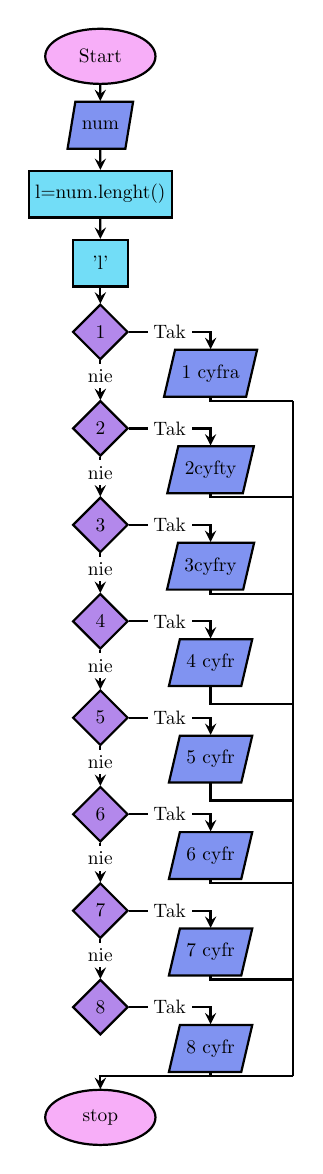
\begin{tikzpicture}[scale=0.7,transform shape]
		\node [style=startstop] (0) at (0, 0) {Start};
		\node [style=io] (1) at (0, -1.25) {num};
		\node [style=process] (3) at (0, -3.75) {'l'};
		\node [style=decision] (4) at (0, -5) {1};
		\node [style=decision] (5) at (0, -6.75) {2};
		\node [style=decision] (6) at (0, -8.5) {3};
		\node [style=decision] (7) at (0, -10.25) {4};
		\node [style=process] (8) at (0, -2.5) {l=num.lenght()};
		\node [style=decision] (9) at (0, -12) {5};
		\node [style=decision] (10) at (0, -13.75) {6};
		\node [style=decision] (11) at (0, -15.5) {7};
		\node [style=decision] (12) at (0, -17.25) {8};
		\node [style=io] (14) at (2, -5.75) {1 cyfra};
		\node [style=io] (15) at (2, -7.5) {2cyfty};
		\node [style=io] (16) at (2, -9.25) {3cyfry};
		\node [style=io] (17) at (2, -11) {4 cyfr};
		\node [style=io] (18) at (2, -12.75) {5 cyfr};
		\node [style=io] (19) at (2, -14.5) {6 cyfr};
		\node [style=io] (20) at (2, -16.25) {7 cyfr};
		\node [style=io] (21) at (2, -18) {8 cyfr};
		\node [style=startstop] (22) at (0, -19.25) {stop};
		\node [style=none] (23) at (3.5, -6.25) {};
		\node [style=none] (24) at (3.5, -8) {};
		\node [style=none] (25) at (3.5, -9.75) {};
		\node [style=none] (26) at (3.5, -11.75) {};
		\node [style=none] (27) at (3.5, -13.5) {};
		\node [style=none] (28) at (3.5, -15) {};
		\node [style=none] (29) at (3.5, -16.75) {};
		\node [style=none] (30) at (3.5, -18.5) {};

%\draw [arrow] (c3) -- (c4)node[pos=0.4,fill=white,inner sep=3]{nie};
%\draw [arrow] (c1) -| (p1)node[pos=0.25,fill=white,inner sep=3]{Tak};

		\draw [style=arrow] (0) to (1);
		\draw [style=arrow] (1) to (8);
		\draw [style=arrow] (8) to (3);
		\draw [style=arrow] (3) to (4);
		\draw [style=arrow] (4) -- (5)node[pos=0.4,fill=white,inner sep=3]{nie};
		\draw [style=arrow] (5) -- (6)node[pos=0.4,fill=white,inner sep=3]{nie};
		\draw [style=arrow] (6) -- (7)node[pos=0.4,fill=white,inner sep=3]{nie};
		\draw [style=arrow] (7) -- (9)node[pos=0.4,fill=white,inner sep=3]{nie};
		\draw [style=arrow] (9) -- (10)node[pos=0.4,fill=white,inner sep=3]{nie};
		\draw [style=arrow] (10) -- (11)node[pos=0.4,fill=white,inner sep=3]{nie};
		\draw [style=arrow] (11) -- (12)node[pos=0.4,fill=white,inner sep=3]{nie};
		\draw [style=arrow] (4) -| (14)node[pos=0.25,fill=white,inner sep=3]{Tak};
		\draw [style=arrow] (5) -| (15)node[pos=0.25,fill=white,inner sep=3]{Tak};
		\draw [style=arrow] (6) -| (16)node[pos=0.25,fill=white,inner sep=3]{Tak};
		\draw [style=arrow] (7) -| (17)node[pos=0.25,fill=white,inner sep=3]{Tak};
		\draw [style=arrow] (9) -| (18)node[pos=0.25,fill=white,inner sep=3]{Tak};
		\draw [style=arrow] (10) -| (19)node[pos=0.25,fill=white,inner sep=3]{Tak};
		\draw [style=arrow] (11) -| (20)node[pos=0.25,fill=white,inner sep=3]{Tak};
		\draw [style=arrow] (12) -| (21)node[pos=0.25,fill=white,inner sep=3]{Tak};
		\draw [style=con] (14) |- (23.center);
		\draw [style=con] (15) |- (24.center);
		\draw [style=con] (16) |- (25.center);
		\draw [style=con] (17) |- (26.center);
		\draw [style=con] (18) |- (27.center);
		\draw [style=con] (19) |- (28.center);
		\draw [style=con] (20) |- (29.center);
		\draw [style=con] (21) |- (30.center);
		\draw [style=con] (23.center) to (30.center);
		\draw [style=arrow] (30.center) -| (22);
\end{tikzpicture}
\caption{2.3 flowchart}
    \label{flow3}
\end{figure}
    \end{flushright}    
\end{multicols}
\subsection*{2.4}
%----------------2.4------------------
\begin{multicols}{2}
  \begin{flushleft}
\begin{minted}[framesep=1mm, baselinestretch=1.,linenos]{python}
print('ile jest liczb podzielnych przez c w <a;b>')
a=int(input('podaj a:'))
b=int(input('podaj b:'))
c=int(input('podaj c:'))
t=bool(a%c)
a=a+(c*t-a%c)
b=b-b%c
n=int((b-a)/c+1)
print(n,' liczb podzielnych przez ',c)
for i in range(0,n):print(a+c*i,',',end="")
\end{minted}
    \end{flushleft}
D:a, dolny limit zakresu $\in$ $\mathbb{Z}$\\
b, górny limit zakresu >a $\in$ $\mathbb{Z}$\\
c, dzielnik $\in$ $\mathbb{Z}$\\
W: strumień, liczby z przedziłu podzielne przez c $\in$ $\mathbb{Z}$
    \begin{flushright}
    \begin{minted}[framesep=1mm, baselinestretch=1.,linenos]{python}
print('ile jest liczb podzielnych przez c w <a;b>')
a=int(input('podaj a:'))
b=int(input('podaj b:'))
c=int(input('podaj c:'))
t=bool(a%c)
a=a+(c*t-a%c)
b=b-b%c
n=int((b-a)/c+1)
print(n,' liczb podzielnych przez ',c)
for i in range(0,n):print(a+c*i,',',end="")
\end{minted}
    \end{flushright}    
\end{multicols}

\subsection*{2.5}
%----------------2.5------------------
\begin{multicols}{2}
  \begin{flushleft}
\begin{minted}[framesep=1mm, baselinestretch=1.,linenos]{python}
print('program do liczenia śrdniej z n liczb')
n=int(input('podaj n:'))
sum=float(0)
for i in range(0,n):
    print('podaj ',i+1,':',end="")
    e=int(input())
    sum=sum+e
sum=round(sum/n,2)
print('średnia',n,'liczba jest równa: ',sum)
\end{minted}
    \end{flushleft}
D: \\
n, ilość liczb $\in$ $\mathbb{N}$\\
e, n'ta liczba ciągu $\in$ $\mathbb{R}$\\
W: strumień, średnia ciągu $\in$ $\mathbb{R}$
    \begin{flushright}
    \begin{minted}[framesep=1mm, baselinestretch=1.,linenos]{python}
print('program do liczenia śrdniej z n liczb')
n=int(input('podaj n:'))
sum=float(0)
for i in range(0,n):
    print('podaj ',i+1,':',end="")
    e=int(input())
    sum=sum+e
sum=round(sum/n,2)
print('średnia',n,'liczba jest równa: ',sum)
\end{minted}
    \end{flushright}    
\end{multicols}

\subsection*{2.6}
%----------------2.6------------------
\begin{multicols}{2}
  \begin{flushleft}
\begin{minted}[framesep=1mm, baselinestretch=1.,linenos]{cpp}
int n=0;cout<<"podaj n: ";cin>>n;
int l[3]= {0,0,0};int p=100;
for (int m=round(pow(75.8531-cos(-0.896604*n),\
cos(0.0903642*n-1.26534))-4.43137);m>0;p++)
{l[0]=floor(p/100);
l[1]=floor((p-l[0]*100)/10);
l[2]=p-(l[1]*10+l[0]*100);
if(l[0]+l[1]+l[2]==n){m--;cout<<p<<endl;}
}cout<<"liczbe możliwości: "<<i;
\end{minted}
    \end{flushleft}
D:n, cyfra $\in$ \{1,2,3...27\}\\
W:strumień, liczby spełniające wrunek\\
i ich ilość $\in$ \{100,101,102...999\}
\begin{flushright}


    \begin{minted}[framesep=1mm, baselinestretch=1.,linenos]{cpp}
int n=0;cout<<"podaj n: ";cin>>n;
int l[3]= {0,0,0};int p=100;
for (int m=round(pow(75.8531-cos(-0.896604*n),\
cos(0.0903642*n-1.26534))-4.43137);m>0;p++)
{l[0]=floor(p/100);
l[1]=floor((p-l[0]*100)/10);
l[2]=p-(l[1]*10+l[0]*100);
if(l[0]+l[1]+l[2]==n){m--;cout<<p<<endl;}
}cout<<"liczbe możliwości: "<<i;
\end{minted}
\end{flushright} 
\end{multicols}

\subsection*{2.7}
%----------------2.7------------------
\begin{multicols}{2}
  \begin{flushleft}
\begin{tikzpicture}
	\begin{pgfonlayer}{nodelayer}
		\node [style=startstop] (0) at (0, 0.25) {Start};
		\node [style=process] (1) at (0, -1.25) {d='N'};
		\node [style=process] (2) at (0, -3) {2.6};
		\node [style=io] (3) at (0, -4.75) {toupper(d)};
		\node [style=decision] (4) at (0, -6.75) {d='T'|| d='N'};
		\node [style=decision] (5) at (1.5, -8.5) {d!='N'};
		\node [style=startstop] (6) at (0, -9.75) {Stop};
		\node [style=none] (7) at (0, -2) {};
		\node [style=none] (8) at (2.75, -2) {};
		\node [style=none] (9) at (-1.75, -3.75) {};
		\node [style=none] (10) at (0, -3.75) {};
	\end{pgfonlayer}
	\begin{pgfonlayer}{edgelayer}
		\draw [style=arrow] (0) to (1);
		\draw [style=arrow] (1) to (2);
		\draw [style=arrow] (2) to (3);
		\draw [style=arrow] (3) to (4);
		\draw [style=arrow] (4) to (5);
		\draw [style=arrow] (5) to (6);
		\draw (5) to (8.center);
		\draw (8.center) to (7.center);
		\draw (4) to (9.center);
		\draw (9.center) to (10.center);
	\end{pgfonlayer}
\end{tikzpicture}

    \end{flushleft}
D:n, cyfra $\in$ \{1,2,3...27\}\\
W:strumień, liczby spełniające wrunek\\
i ich ilość $\in$ \{100,101,102...999\}
    \begin{flushright}
    \renewcommand{\thefigure}{7}
\begin{figure}[H]
    \centering 
    %text width=1cm
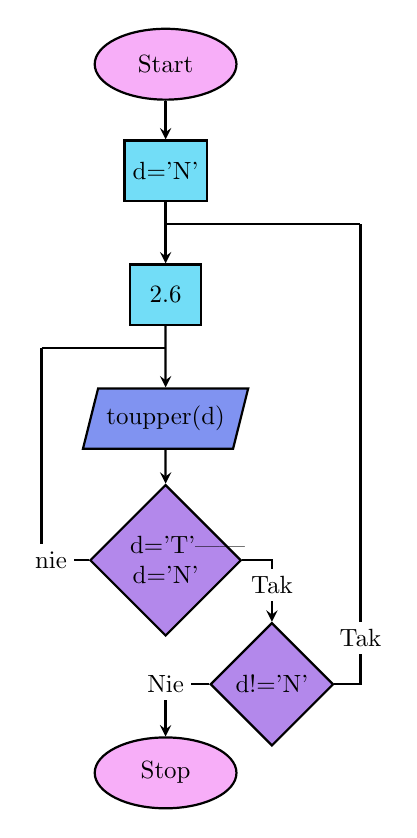
\begin{tikzpicture}[scale=0.9,transform shape]
		\node [style=startstop] (0) at (0, 0.25) {Start};
		\node [style=process] (1) at (0, -1.25) {d='N'};
		\node [style=process] (2) at (0, -3) {2.6};
		\node [style=io] (3) at (0, -4.75) {toupper(d)};
		\node [style=decision,text width=1cm] (4) at (0, -6.75) {d='T'|| d='N'};
		\node [style=decision] (5) at (1.5, -8.5) {d!='N'};
		\node [style=startstop] (6) at (0, -9.75) {Stop};
		\node [style=none] (7) at (0, -2) {};
		\node [style=none] (8) at (2.75, -2) {};
		\node [style=none] (9) at (-1.75, -3.75) {};
		\node [style=none] (10) at (0, -3.75) {};

        % node[pos=0.4,fill=white,inner sep=3]{Nie};
		% node[pos=0.25,fill=white,inner sep=3]{Tak};

		\draw [style=arrow] (0) to (1);
		\draw [style=arrow] (1) to (2);
		\draw [style=arrow] (2) to (3);
		\draw [style=arrow] (3) to (4);
		\draw [style=arrow] (4) -| (5)node[pos=0.7,fill=white,inner sep=3]{Tak};
		\draw [style=arrow] (5) -| (6)node[pos=0.5,fill=white,inner sep=3]{Nie};
		\draw [style=con] (5) -| (8.center)node[pos=0.55,fill=white,inner sep=3]{Tak};
		\draw [style=con] (8.center) to (7.center);
		\draw [style=con] (4) -| (9.center)node[pos=0.4,fill=white,inner sep=3]{nie};
		\draw [style=con] (9.center) to (10.center);     
\end{tikzpicture}
\caption{2.7 flowchart}
    \label{flow7}
\end{figure}
    \end{flushright}    
\end{multicols}

\subsection*{2.8}
%----------------2.8------------------
\begin{multicols}{2}
  \begin{flushleft}
\renewcommand{\thefigure}{8}
\begin{figure}[H]
    \centering 
    %text width=1cm
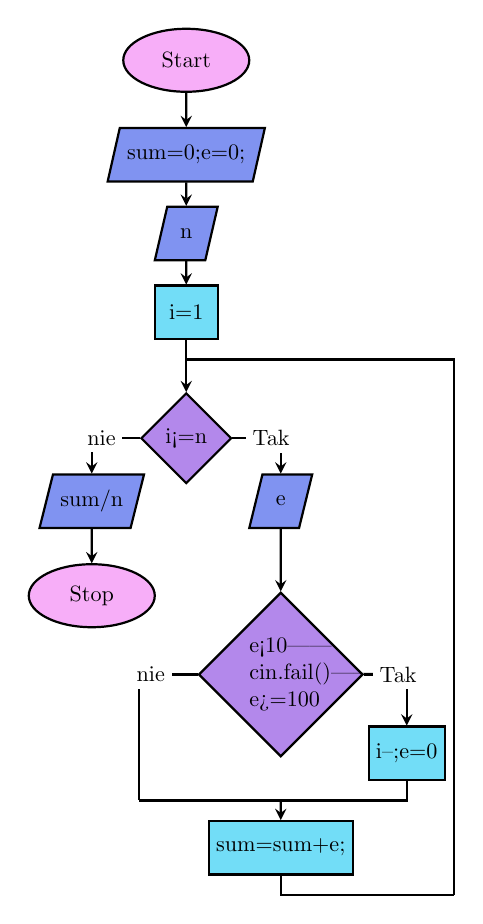
\begin{tikzpicture}[scale=0.8,transform shape]
		\node [style=startstop] (0) at (0, 0) {Start};
		\node [style=io] (1) at (0, -1.5) {sum=0;e=0;};
		\node [style=io] (2) at (0, -2.75) {n};
		\node [style=process] (3) at (0, -4) {i=1};
		\node [style=decision] (4) at (0, -6) {i<=n};
		\node [style=io] (5) at (1.5, -7) {e};
		\node [style=decision,text width=1cm] (6) at (1.5, -9.75) {e<10|| cin.fail()||  e>=100};
		\node [style=process] (7) at (3.5, -11) {i--;e=0};
		\node [style=process] (8) at (1.5, -12.5) {sum=sum+e;};
		\node [style=none] (9) at (1.5, -11.75) {};
		\node [style=none] (10) at (-0.75, -11.75) {};
		\node [style=none] (11) at (4.25, -13.25) {};
		\node [style=none] (12) at (0, -4.75) {};
		\node [style=io] (13) at (-1.5, -7) {sum/n};
		\node [style=startstop] (14) at (-1.5, -8.5) {Stop};

        % node[pos=0.4,fill=white,inner sep=3]{nie};
		% node[pos=0.25,fill=white,inner sep=3]{Tak};
        
		\draw [style=arrow] (2) to (3);
		\draw [style=arrow] (3) to (4);
		\draw [style=arrow] (4) -| (5)node[pos=0.4,fill=white,inner sep=3]{Tak};
		\draw [style=arrow] (5) to (6);
		\draw [style=arrow] (6) -| (7)node[pos=0.4,fill=white,inner sep=3]{Tak};
		\draw [style=con] (7) |- (9.center);
		\draw [style=con] (6) -| (10.center)node[pos=0.4,fill=white,inner sep=3]{nie};
		\draw [style=con] (10.center) to (9.center);
		\draw [style=arrow] (9.center) to (8);
		\draw [style=con] (8) |- (11.center);
		\draw [style=con] (11.center) |- (12.center);
		\draw [style=arrow] (0) to (1);
		\draw [style=arrow] (1) to (2);
		\draw [style=arrow] (4) -| (13)node[pos=0.4,fill=white,inner sep=3]{nie};
		\draw [style=arrow] (13) to (14);

\end{tikzpicture}
\caption{2.8 flowchart}
    \label{flow8}
\end{figure}
    \end{flushleft}
D: \\
n, ilość liczb $\in$ $\mathbb{N}$\\
e, n'ta liczba ciągu $\in$ \{10,11,12...99\}\\
W: strumień, średnia ciągu $\in$ $\mathbb{R}$
    \begin{flushright}
    \renewcommand{\thefigure}{8}
\begin{figure}[H]
    \centering 
    %text width=1cm
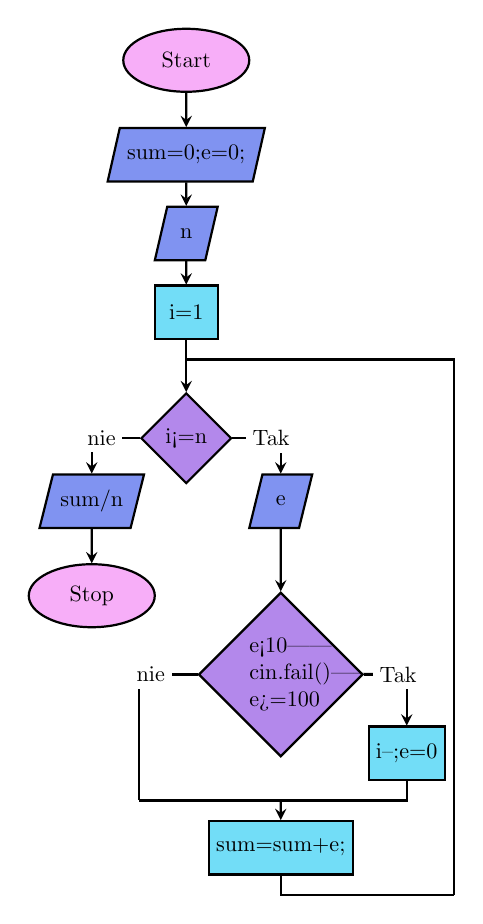
\begin{tikzpicture}[scale=0.8,transform shape]
		\node [style=startstop] (0) at (0, 0) {Start};
		\node [style=io] (1) at (0, -1.5) {sum=0;e=0;};
		\node [style=io] (2) at (0, -2.75) {n};
		\node [style=process] (3) at (0, -4) {i=1};
		\node [style=decision] (4) at (0, -6) {i<=n};
		\node [style=io] (5) at (1.5, -7) {e};
		\node [style=decision,text width=1cm] (6) at (1.5, -9.75) {e<10|| cin.fail()||  e>=100};
		\node [style=process] (7) at (3.5, -11) {i--;e=0};
		\node [style=process] (8) at (1.5, -12.5) {sum=sum+e;};
		\node [style=none] (9) at (1.5, -11.75) {};
		\node [style=none] (10) at (-0.75, -11.75) {};
		\node [style=none] (11) at (4.25, -13.25) {};
		\node [style=none] (12) at (0, -4.75) {};
		\node [style=io] (13) at (-1.5, -7) {sum/n};
		\node [style=startstop] (14) at (-1.5, -8.5) {Stop};

        % node[pos=0.4,fill=white,inner sep=3]{nie};
		% node[pos=0.25,fill=white,inner sep=3]{Tak};
        
		\draw [style=arrow] (2) to (3);
		\draw [style=arrow] (3) to (4);
		\draw [style=arrow] (4) -| (5)node[pos=0.4,fill=white,inner sep=3]{Tak};
		\draw [style=arrow] (5) to (6);
		\draw [style=arrow] (6) -| (7)node[pos=0.4,fill=white,inner sep=3]{Tak};
		\draw [style=con] (7) |- (9.center);
		\draw [style=con] (6) -| (10.center)node[pos=0.4,fill=white,inner sep=3]{nie};
		\draw [style=con] (10.center) to (9.center);
		\draw [style=arrow] (9.center) to (8);
		\draw [style=con] (8) |- (11.center);
		\draw [style=con] (11.center) |- (12.center);
		\draw [style=arrow] (0) to (1);
		\draw [style=arrow] (1) to (2);
		\draw [style=arrow] (4) -| (13)node[pos=0.4,fill=white,inner sep=3]{nie};
		\draw [style=arrow] (13) to (14);

\end{tikzpicture}
\caption{2.8 flowchart}
    \label{flow8}
\end{figure}
    \end{flushright}    
\end{multicols}

\subsection*{2.9}
%----------------2.9------------------
\begin{multicols}{2}
  \begin{flushleft}
\renewcommand{\thefigure}{9}
\begin{figure}[H]
    \centering 
    %text width=1cm
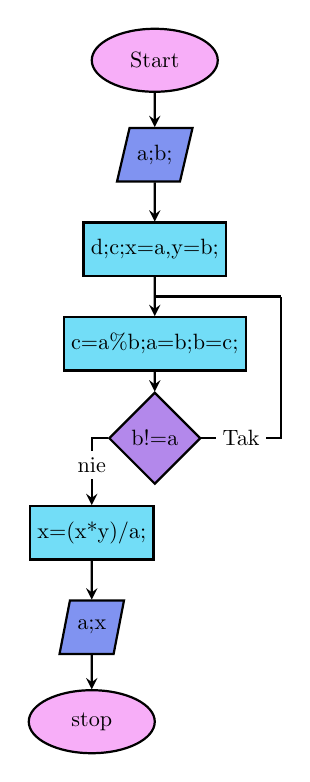
\begin{tikzpicture}[scale=0.8,transform shape]
        \node [style=startstop] (0) at (0, 0) {Start};
		\node [style=io] (1) at (0, -1.5) {a;b;};
		\node [style=process] (2) at (0, -3) {d;c;x=a,y=b;};
		\node [style=process] (3) at (0, -4.5) {c=a\%b;a=b;b=c;};
		\node [style=decision] (4) at (0, -6) {b!=a};
		\node [style=none] (5) at (2, -3.75) {};
		\node [style=none] (6) at (0, -3.75) {};
		\node [style=process] (7) at (-1, -7.5) {x=(x*y)/a;};
		\node [style=io] (8) at (-1, -9) {a;x};
		\node [style=startstop] (9) at (-1, -10.5) {stop};

        % node[pos=0.4,fill=white,inner sep=3]{nie};
		% node[pos=0.25,fill=white,inner sep=3]{Tak};

		\draw [style=arrow] (0) to (1);
		\draw [style=arrow] (1) to (2);
		\draw [style=arrow] (2) to (3);
		\draw [style=arrow] (3) to (4);
		\draw [style=arrow] (8) to (9);
		\draw [style=con] (4) -| (5.center)node[pos=0.25,fill=white,inner sep=3]{Tak};
		\draw [style=con] (5.center) to (6.center);
		\draw [style=arrow] (4) -| (7)node[pos=0.7,fill=white,inner sep=3]{nie};
		\draw [style=arrow] (7) to (8);
\end{tikzpicture}
\caption{2.9 flowchart}
    \label{flow9}
\end{figure}
    \end{flushleft}
D:a i b, liczby do nww i nwd $\in$ $\mathbb{N}$\\
W:a i x, nww i nwd $\in$ $\mathbb{N}$
    \begin{flushright}
    \renewcommand{\thefigure}{9}
\begin{figure}[H]
    \centering 
    %text width=1cm
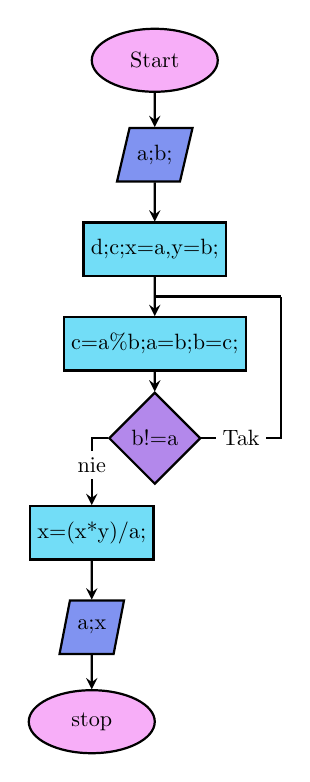
\begin{tikzpicture}[scale=0.8,transform shape]
        \node [style=startstop] (0) at (0, 0) {Start};
		\node [style=io] (1) at (0, -1.5) {a;b;};
		\node [style=process] (2) at (0, -3) {d;c;x=a,y=b;};
		\node [style=process] (3) at (0, -4.5) {c=a\%b;a=b;b=c;};
		\node [style=decision] (4) at (0, -6) {b!=a};
		\node [style=none] (5) at (2, -3.75) {};
		\node [style=none] (6) at (0, -3.75) {};
		\node [style=process] (7) at (-1, -7.5) {x=(x*y)/a;};
		\node [style=io] (8) at (-1, -9) {a;x};
		\node [style=startstop] (9) at (-1, -10.5) {stop};

        % node[pos=0.4,fill=white,inner sep=3]{nie};
		% node[pos=0.25,fill=white,inner sep=3]{Tak};

		\draw [style=arrow] (0) to (1);
		\draw [style=arrow] (1) to (2);
		\draw [style=arrow] (2) to (3);
		\draw [style=arrow] (3) to (4);
		\draw [style=arrow] (8) to (9);
		\draw [style=con] (4) -| (5.center)node[pos=0.25,fill=white,inner sep=3]{Tak};
		\draw [style=con] (5.center) to (6.center);
		\draw [style=arrow] (4) -| (7)node[pos=0.7,fill=white,inner sep=3]{nie};
		\draw [style=arrow] (7) to (8);
\end{tikzpicture}
\caption{2.9 flowchart}
    \label{flow9}
\end{figure}
    \end{flushright}    
\end{multicols}

\subsection*{2.10}
%----------------2.10------------------
\begin{multicols}{2}
  \begin{flushleft}
\begin{minted}[framesep=1mm, baselinestretch=1.,linenos]{cpp}
int a[2]={0,16};
string c[2]={"min","max"};
int i;int x;int y;int l=4;
cout<<"program tabliczka mno�enie od do.\n\
Program przymuje wartości <-15;15>"<<endl;  
while(i<2){
cout<<"podaj "<<c[i]<<": ";
cin.clear();cin.sync();
a[i]=0;cin>>a[i];
if(cin.fail()||abs(a[i])>15||a[0]>a[1])
{cout<<endl<<"podana wartość jest nie poprawna"<<endl;
i--;}i++;}system("cls");y=a[0];
while (y<=a[1])
{
    x=a[0];cout<<y;gotoxy(3,y-a[0]+2);
    cout<<"|";
    while (x<=a[1]){
        gotoxy((x-a[0]+1)*l,y-a[0]+2);
        cout<<y*x;
        x++;}
    cout<<endl;y++;
}
\end{minted}
    \end{flushleft}
D: a[], przedział tabliczki mnożenia $\in$ \{-15,-14,-13...15\}\\
W: strumień, tabliczka mnożenia od a[0] do a[1] $\in$ \{-225,-224,-223...225\}
    \begin{flushright}
    \begin{minted}[framesep=1mm, baselinestretch=1.,linenos]{cpp}
int a[2]={0,16};
string c[2]={"min","max"};
int i;int x;int y;int l=4;
cout<<"program tabliczka mno�enie od do.\n\
Program przymuje wartości <-15;15>"<<endl;  
while(i<2){
cout<<"podaj "<<c[i]<<": ";
cin.clear();cin.sync();
a[i]=0;cin>>a[i];
if(cin.fail()||abs(a[i])>15||a[0]>a[1])
{cout<<endl<<"podana wartość jest nie poprawna"<<endl;
i--;}i++;}system("cls");y=a[0];
while (y<=a[1])
{
    x=a[0];cout<<y;gotoxy(3,y-a[0]+2);
    cout<<"|";
    while (x<=a[1]){
        gotoxy((x-a[0]+1)*l,y-a[0]+2);
        cout<<y*x;
        x++;}
    cout<<endl;y++;
}
\end{minted}
    \end{flushright}    
\end{multicols}
\newpage

\subsection*{2.11}
%----------------2.11------------------
\begin{multicols}{2}
  \begin{flushleft}
\begin{minted}[framesep=1mm, baselinestretch=1.,linenos]{cpp}
int i;int a;int min=100;
cout<<"program do szukania minimalne liczby\
z ciągu liczb dwu cyfrowych"<<endl;  
cout<<"aby zakończyć podawanie ciągu\
podaj liczbę 0"<<endl;  
while(a!=0)
{  
i++;cin.clear();cin.sync();
cout<<"podaj "<<i<<":";
a=0;cin>>a;        
if(a==0){break;}
else if(cin.fail()||abs(a)<10||abs(a)>99)
{cout<<"podana wartość jest nie poprawna"\
<<endl;i--;}
else{if(a<min){min=a;}}
}
cout<<"minimalną liczbą z ciągu:"<<endl;
if(min==100)
{cout<<"najmniejsza liczba ci¹gu nale¿y\
do zbioru pustego"<<endl;}
else{cout<<endl<<"jest: "<<min<<endl;}
\end{minted}
    \end{flushleft}
D: a, n'ta liczba ciągu $\in$ $\mathbb{R}$\\
W: min, najmniejszu element ciągu $\in$ $\mathbb{R}$
    \begin{flushright}
    \begin{minted}[framesep=1mm, baselinestretch=1.,linenos]{cpp}
int i;int a;int min=100;
cout<<"program do szukania minimalne liczby\
z ciągu liczb dwu cyfrowych"<<endl;  
cout<<"aby zakończyć podawanie ciągu\
podaj liczbę 0"<<endl;  
while(a!=0)
{  
i++;cin.clear();cin.sync();
cout<<"podaj "<<i<<":";
a=0;cin>>a;        
if(a==0){break;}
else if(cin.fail()||abs(a)<10||abs(a)>99)
{cout<<"podana wartość jest nie poprawna"\
<<endl;i--;}
else{if(a<min){min=a;}}
}
cout<<"minimalną liczbą z ciągu:"<<endl;
if(min==100)
{cout<<"najmniejsza liczba ci¹gu nale¿y\
do zbioru pustego"<<endl;}
else{cout<<endl<<"jest: "<<min<<endl;}
\end{minted}
    \end{flushright}    
\end{multicols}

\subsection*{2.12}
%----------------2.12------------------
\begin{multicols}{2}
  \begin{flushleft}
\begin{minted}[framesep=1mm, baselinestretch=1.,linenos]{cpp}
cout<<"program do nwd i nww"<<endl;  
int i;
char l='a';
int g[2]={0,0};      
while(i<2){
cout<<"podaj "<<l<<": ";
cin.clear();cin.sync();
g[i]=0;cin>>g[i];
if(cin.fail())
{cout<<endl<<"podana wartość jest nie poprawna"\
<<endl;i--;l--;}
i++;l++;}	
int a=abs(g[0]);int x=a;
int b=abs(g[1]);int y=b;     
while(a!=b)
{
	if(a>b){a=a-b;}
	else{b=b-a;}
}
x=(x*y)/a;
cout<<"nwd:"<<a<<" nww:"<<x<<endl;
\end{minted}
    \end{flushleft}
D:a i b, liczby do nww i nwd $\in$ $\mathbb{N}$\\
W:a i x, nww i nwd $\in$ $\mathbb{N}$
    \begin{flushright}
    \begin{minted}[framesep=1mm, baselinestretch=1.,linenos]{cpp}
cout<<"program do nwd i nww"<<endl;  
int i;
char l='a';
int g[2]={0,0};      
while(i<2){
cout<<"podaj "<<l<<": ";
cin.clear();cin.sync();
g[i]=0;cin>>g[i];
if(cin.fail())
{cout<<endl<<"podana wartość jest nie poprawna"\
<<endl;i--;l--;}
i++;l++;}	
int a=abs(g[0]);int x=a;
int b=abs(g[1]);int y=b;     
while(a!=b)
{
	if(a>b){a=a-b;}
	else{b=b-a;}
}
x=(x*y)/a;
cout<<"nwd:"<<a<<" nww:"<<x<<endl;
\end{minted}
    \end{flushright}    
\end{multicols}
\newpage
\subsection*{2.13}
%----------------2.13------------------
\begin{multicols}{2}
  \begin{flushleft}
  \begin{minted}[framesep=1mm, baselinestretch=1.,linenos]{cpp}
cout<<"program liczenia silni z n"<<endl;   
int i;int n;long long s;
i=1;n=1;s=1;
cout<<"podaj n:";
cin.clear();cin.sync();cin>>n;
while(i<=n){s=s*i;i++;}
cout<<"silna z n jest równa:"<<s<<endl;
\end{minted}
D: n, liczba do silni $\in$ $\mathbb{N}$\\
W: s, silnia n $\in$ $\mathbb{N}$
\begin{minted}[framesep=1mm, baselinestretch=1.,linenos]{text}
Zarezerwuj miejsce dla i, n, s
i, n, s równają się 1 
Zapytaj użytkownika o n
s jest równe iloczynowi i oraz s
zwiększ i o jeden
jeżeli i jest nie mniejsze od n wróć do pkt.4
przekaż s do strumienia  
\end{minted}
    \end{flushleft}

    \begin{flushright}
    \begin{minted}[framesep=1mm, baselinestretch=1.,linenos]{cpp}
cout<<"program liczenia silni z n"<<endl;   
int i;int n;long long s;
i=1;n=1;s=1;
cout<<"podaj n:";
cin.clear();cin.sync();cin>>n;
while(i<=n){s=s*i;i++;}
cout<<"silna z n jest równa:"<<s<<endl;
\end{minted}
    \end{flushright}    
\end{multicols}

\subsection*{2.14}
%----------------2.14------------------
\begin{multicols}{2}
  \begin{flushleft}
\begin{minted}[framesep=1mm, baselinestretch=1.,linenos]{cpp}
cout<<endl<<"program do liczenie n liczby fibonacciego"<<endl;  
cout<<"\npodaj n:";
int n = 0;
cin>>n;
if(cin.fail()){r=false;cout<<endl<<"podana wartość jest nie poprawna"<<endl;}
int i = 0;
double a=0;double b=1;double c=0;
while (n>i)
{c=a+b;a=b;b=c;i++;}
cout<<n<<" liczba ciagu fibonacciego jest rowna:"<<a<<endl;
\end{minted}
D: n, index liczby fibonaciego $\in$ $\mathbb{N}$\\
W: s, n'ta liczba ciągu fibonaciego $\in$ $\mathbb{N}$
\end{flushleft}
\begin{minipage}{3cm}
%\vspace{1cm}
\begin{minted}[framesep=1mm, baselinestretch=1.,linenos]{text}
Zarezerwuj miejsce dla n, i, a, b, c
b równa się 1 
c jest równe sumie a i b
a równa się b
b równa się c 
zwiększ i o jeden
jeżeli n jest większe od i to wróć do 3 kroku
przekaż a do strumienia
\end{minted}   
\end{minipage}
\begin{flushright}
\end{flushright}    
\end{multicols}
\hspace{3cm}
\begin{minipage}{3cm}
\begin{minted}[framesep=1mm, baselinestretch=1.,linenos]{cpp}
cout<<endl<<"program do liczenie n liczby fibonacciego"<<endl;  
cout<<"\npodaj n:";
int n = 0;
cin>>n;
if(cin.fail()){r=false;cout<<endl<<"podana wartość jest nie poprawna"<<endl;}
int i = 0;
double a=0;double b=1;double c=0;
while (n>i)
{c=a+b;a=b;b=c;i++;}
cout<<n<<" liczba ciagu fibonacciego jest rowna:"<<a<<endl;
\end{minted}  
\end{minipage}

    


\newpage
\subsection*{2.15}
%----------------2.15------------------
\begin{multicols}{2}
  \begin{flushleft}


D: n, liczba do sprawdzenia $\in$ $\mathbb{N}$\\
W: odp, czy liczba jest pierwsza $\in$ $\{"tak";"nie"\}$

\hspace{0.4cm}
\begin{minipage}{3cm}
\vspace{0.6cm}
\small
\begin{minted}[framesep=1mm, baselinestretch=1.,linenos]{text}
Odp równa się „tak”, i równa się 3 a n równa się jeden
Zapytaj użytkownika o n
Jeżeli  n jest podzielne przez 2 to odp przyjmuje wartość „nie”
Jeżeli reszta n/i jest 0 to odp przyjmuje wartość „nie”
Zwiększ i o 2
Jeżeli i jest mniejszy od pierwiastku z n to idź do czwartego kroku 
Przekaż odp do strumienia 
\end{minted}
\normalsize
\begin{minted}[framesep=1mm, baselinestretch=1.,linenos]{python}
import math
print('sprawdzanie czy liczba jest pierwsza')
i=int(2)
n=int(1)
odp='tak'
while True:
    try:
        n=int(input('podaj a liczbe:'))
        break   
    except ValueError:print('zła wartość')

while i<=math.sqrt(n):
    if n%i==0:
        odp='nie'
        break
    i=i+1
print(odp)
\end{minted}
\end{minipage}

    \end{flushleft}

    \begin{flushright}
    \begin{minted}[framesep=1mm, baselinestretch=1.,linenos]{python}
import math
print('sprawdzanie czy liczba jest pierwsza')
i=int(2)
n=int(1)
odp='tak'
while True:
    try:
        n=int(input('podaj a liczbe:'))
        break   
    except ValueError:print('zła wartość')

while i<=math.sqrt(n):
    if n%i==0:
        odp='nie'
        break
    i=i+1
print(odp)
\end{minted}
   
    \end{flushright}    
\end{multicols}
\subsection*{2.16}

%----------------2.16------------------
\normalsize
\begin{multicols}{2}
  \begin{flushleft}
D: n, liczba $\in$ $\mathbb{N}_0$\\
W: s, ilość cyfr w n $\in$ $\mathbb{N}_0$

\hspace{0.4cm}
\begin{minipage}{3cm}
\vspace{0.6cm}
\begin{minted}[framesep=1mm, baselinestretch=1.,linenos]{text}
Zarezerwuj miejsce dla n i s 
Zapytaj użytkownika o n
Dodaj do s resztę dzielenia dziesiętnego z n
Podziel n przez dziesięć 
Jeżeli n nie równa się zero idź do kroku 3
Przekaż s do strumienia 
\end{minted}
\renewcommand{\thefigure}{16}
\begin{figure}[H]
    \centering 
    %text width=1cm
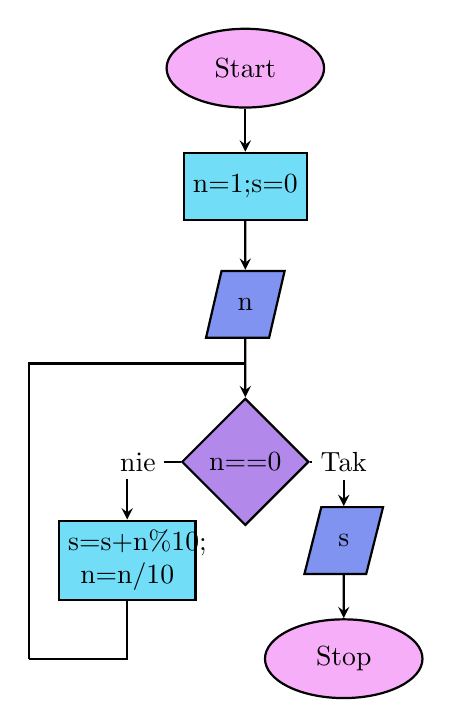
\begin{tikzpicture}
	    \node [style=startstop] (0) at (0, 0) {Start};
		\node [style=process] (1) at (0, -1.5) {n=1;s=0};
		\node [style=io] (2) at (0, -3) {n};
		\node [style=decision] (3) at (0, -5) {n==0};
		\node [style=io] (4) at (1.25, -6) {s};
		\node [style=startstop] (5) at (1.25, -7.5) {Stop};
		\node [style=process,text width=1.5cm] (6) at (-1.5, -6.25) {s=s+n\%10; n=n/10};
		\node [style=none] (7) at (-2.75, -7.5) {};
		\node [style=none] (8) at (0, -3.75) {};

        % node[pos=0.4,fill=white,inner sep=3]{nie};
		% node[pos=0.25,fill=white,inner sep=3]{Tak};

		\draw [style=arrow] (0) to (1);
		\draw [style=arrow] (1) to (2);
		\draw [style=arrow] (2) to (3);
		\draw [style=arrow] (3) -| (4)node[pos=0.5,fill=white,inner sep=3]{Tak};
		\draw [style=arrow] (4) to (5);
		\draw [style=arrow] (3) -| (6)node[pos=0.4,fill=white,inner sep=3]{nie};
		\draw [style=con] (6) |- (7.center);
		\draw [style=con] (7.center) |- (8.center);
\end{tikzpicture}
\caption{2.16 flowchart}
    \label{flow16}
\end{figure}
\end{minipage}


    \end{flushleft}

    \begin{flushright}
    
    \begin{tikzpicture}
	\begin{pgfonlayer}{nodelayer}
		\node [style=startstop] (0) at (0, 0) {Start};
		\node [style=process] (1) at (0, -1.5) {n=1;s=0};
		\node [style=io] (2) at (0, -3) {n};
		\node [style=decision] (3) at (0, -5) {n==0};
		\node [style=io] (4) at (1.25, -6) {s};
		\node [style=startstop] (5) at (1.25, -7.5) {Stop};
		\node [style=process] (6) at (-1.5, -6.25) {s=s+n\%10; n=n/10};
		\node [style=none] (7) at (-2.75, -7.5) {};
		\node [style=none] (8) at (0, -3.75) {};
	\end{pgfonlayer}
	\begin{pgfonlayer}{edgelayer}
		\draw [style=arrow] (0) to (1);
		\draw [style=arrow] (1) to (2);
		\draw [style=arrow] (2) to (3);
		\draw [style=arrow] (3) to (4);
		\draw [style=arrow] (4) to (5);
		\draw [style=arrow] (3) to (6);
		\draw [style=con] (6) to (7.center);
		\draw [style=con] (7.center) to (8.center);
	\end{pgfonlayer}
\end{tikzpicture}

    \end{flushright}    
\end{multicols}
\newpage
%-------------alternatywne rozwiązamnia
\section{Alternatywne rozwiązania}
\begin{center}
\large \textbf{python}
\end{center}
\small
\begin{multicols}{2}
\begin{flushleft}
    \hspace{1cm}
    \begin{minipage}{3cm}
        \subsection*{2.1}
        \renewcommand{\thefigure}{1}
\begin{figure}[H]
  \centering  
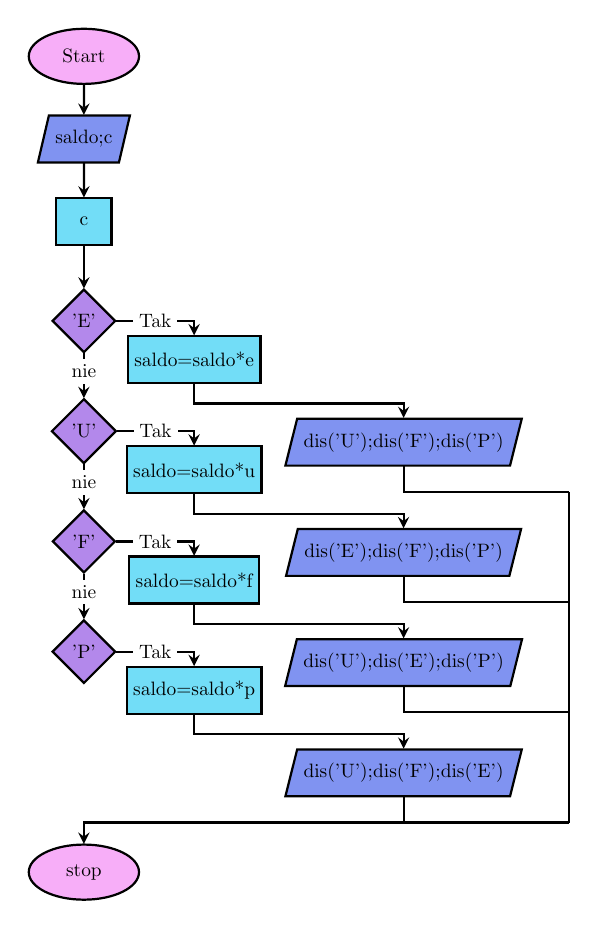
\begin{tikzpicture}[scale=0.7,transform shape,node distance=1.5cm]

\node (start) [startstop] {Start};
\node (in1) [io, below of=start] {saldo;c};
\node (s1) [process, below of=in1] {c};

\node (c1) [decision, below of=s1,yshift=-0.3cm] {'E'};
\node (p1) [process, below of=c1, xshift=2cm,yshift=0.8cm] {saldo=saldo*e};
\node (out1) [io, right of=p1, xshift=2.3cm, yshift=-1.5cm] {dis('U');dis('F');dis('P')};

\node (c2) [decision, below of=c1,yshift=-0.5cm] {'U'};
\node (p2) [process, below of=c2, xshift=2cm,yshift=0.8cm] {saldo=saldo*u};
\node (out2) [io, right of=p2, xshift=2.3cm, yshift=-1.5cm] {dis('E');dis('F');dis('P')};

\node (c3) [decision, below of=c2,yshift=-0.5cm] {'F'};
\node (p3) [process, below of=c3, xshift=2cm,yshift=0.8cm] {saldo=saldo*f};
\node (out3) [io, right of=p3, xshift=2.3cm, yshift=-1.5cm] {dis('U');dis('E');dis('P')};

\node (c4) [decision, below of=c3,yshift=-0.5cm] {'P'};
\node (p4) [process, below of=c4, xshift=2cm,yshift=0.8cm] {saldo=saldo*p};
\node (out4) [io, right of=p4, xshift=2.3cm, yshift=-1.5cm] {dis('U');dis('F');dis('E')};

\node (e1)[coordinate,below of=c1,xshift=4.5cm]{};
\node (e2)[coordinate,below of=c2,xshift=4.5cm]{};
\node (e3)[coordinate,below of=c3,xshift=4.5cm]{};
\node (e4)[coordinate,below of=c4,xshift=4.5cm]{};
\node (e5)[coordinate,below of=out1,yshift=0.6cm,xshift=3cm]{};
\node (e6)[coordinate,below of=out2,yshift=0.6cm,xshift=3cm]{};
\node (e7)[coordinate,below of=out3,yshift=0.6cm,xshift=3cm]{};
\node (e8)[coordinate,below of=out4,yshift=0.6cm,xshift=3cm]{};

\node (stop) [startstop, below of =c4,yshift=-2.5cm]{stop};

\draw [arrow] (start) -- (in1);
\draw [arrow] (in1) -- (s1);
\draw [arrow] (s1) -- (c1);
\draw [arrow] (c1) -- (c2)node[pos=0.4,fill=white,inner sep=3]{nie};
\draw [arrow] (c2) -- (c3)node[pos=0.4,fill=white,inner sep=3]{nie};
\draw [arrow] (c3) -- (c4)node[pos=0.4,fill=white,inner sep=3]{nie};
\draw [arrow] (c1) -| (p1)node[pos=0.25,fill=white,inner sep=3]{Tak};
\draw [arrow] (c2) -| (p2)node[pos=0.25,fill=white,inner sep=3]{Tak};
\draw [arrow] (c3) -| (p3)node[pos=0.25,fill=white,inner sep=3]{Tak};
\draw [arrow] (c4) -| (p4)node[pos=0.25,fill=white,inner sep=3]{Tak};

\draw [thick] (p1) |- (e1);
\draw [thick] (p2) |- (e2);
\draw [thick] (p3) |- (e3);
\draw [thick] (p4) |- (e4);

\draw [arrow] (e1) -| (out1);
\draw [arrow] (e2) -| (out2);
\draw [arrow] (e3) -| (out3);
\draw [arrow] (e4) -| (out4);

\draw [thick] (out1) |- (e5);
\draw [thick] (out2) |- (e6);
\draw [thick] (out3) |- (e7);
\draw [thick] (out4) |- (e8);

\draw [thick] (e5) |- (e8);


\draw [arrow] (e8) -| (stop);


\end{tikzpicture}
    \caption{2.1 flowchart}
    \label{flow1}
\end{figure}
    

        \subsection*{2.2}
        \renewcommand{\thefigure}{2}
\begin{figure}[H]
    \centering  
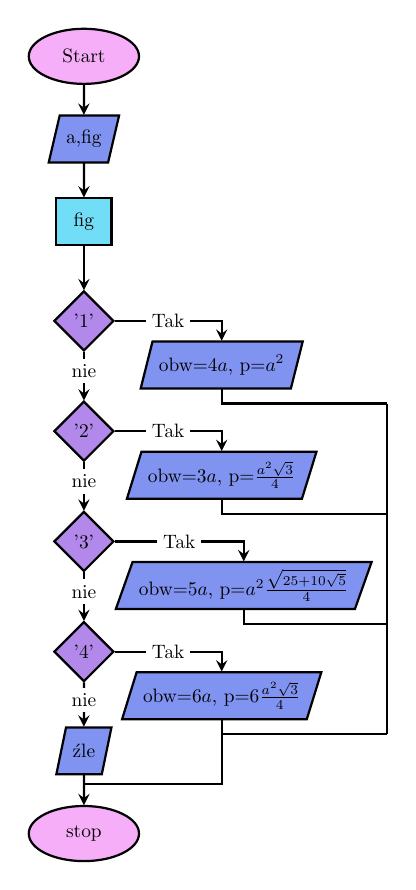
\begin{tikzpicture}[scale=0.7,transform shape,node distance=1.5cm]

\node (start) [startstop] {Start};
\node (in1) [io, below of=start] {a,fig};
\node (s1) [process, below of=in1] {fig};

\node (c1) [decision, below of=s1,yshift=-0.3cm] {'1'};
\node (out1) [io, right of=c1, xshift=1cm, yshift=-0.8cm] {obw=$4a$, p=$a^2$};

\node (c2) [decision, below of=c1,yshift=-0.5cm] {'2'};
\node (out2) [io, right of=c2, xshift=1cm, yshift=-0.8cm] {obw=$3a$, p=$\frac{a^2\sqrt{3}}{4}$};

\node (c3) [decision, below of=c2,yshift=-0.5cm] {'3'};
\node (out3) [io, right of=c3, xshift=1.4cm, yshift=-0.8cm] {obw=$5a$, p=$a^2\frac{\sqrt{25+10\sqrt{5}}}{4}$};

\node (c4) [decision, below of=c3,yshift=-0.5cm] {'4'};
\node (out4) [io, right of=c4, xshift=1cm, yshift=-0.8cm] {obw=$6a$, p=$6\frac{a^2\sqrt{3}}{4}$};

\node (c5) [io, below of=c4, yshift=-0.3cm] {źle};

\node (e1)[coordinate,below of=c1,xshift=5.5cm]{};
\node (e2)[coordinate,below of=c2,xshift=5.5cm]{};
\node (e3)[coordinate,below of=c3,xshift=5.5cm]{};
\node (e4)[coordinate,below of=c4,xshift=5.5cm]{};
\node (e5)[coordinate,below of=c5,yshift=0.9cm]{};

\node (stop) [startstop, below of =c5,yshift=0cm]{stop};

\draw [arrow] (start) -- (in1);
\draw [arrow] (in1) -- (s1);
\draw [arrow] (s1) -- (c1);

\draw [arrow] (c1) -- (c2)node[pos=0.4,fill=white,inner sep=3]{nie};
\draw [arrow] (c2) -- (c3)node[pos=0.4,fill=white,inner sep=3]{nie};
\draw [arrow] (c3) -- (c4)node[pos=0.4,fill=white,inner sep=3]{nie};
\draw [arrow] (c4) -- (c5)node[pos=0.4,fill=white,inner sep=3]{nie};
\draw [arrow] (c1) -| (out1)node[pos=0.25,fill=white,inner sep=3]{Tak};
\draw [arrow] (c2) -| (out2)node[pos=0.25,fill=white,inner sep=3]{Tak};
\draw [arrow] (c3) -| (out3)node[pos=0.25,fill=white,inner sep=3]{Tak};
\draw [arrow] (c4) -| (out4)node[pos=0.25,fill=white,inner sep=3]{Tak};

\draw [thick] (out1) |- (e1);
\draw [thick] (out2) |- (e2);
\draw [thick] (out3) |- (e3);
\draw [thick] (out4) |- (e4);

\draw [thick] (e1) |- (e4);
\draw [thick] (out4) |- (e5);

\draw [arrow] (c5) -- (stop);

\end{tikzpicture}
    \caption{2.2 flowchart}
    \label{flow2}
\end{figure}


        \subsection*{2.3}
        \renewcommand{\thefigure}{3}
\begin{figure}[H]
    \centering 
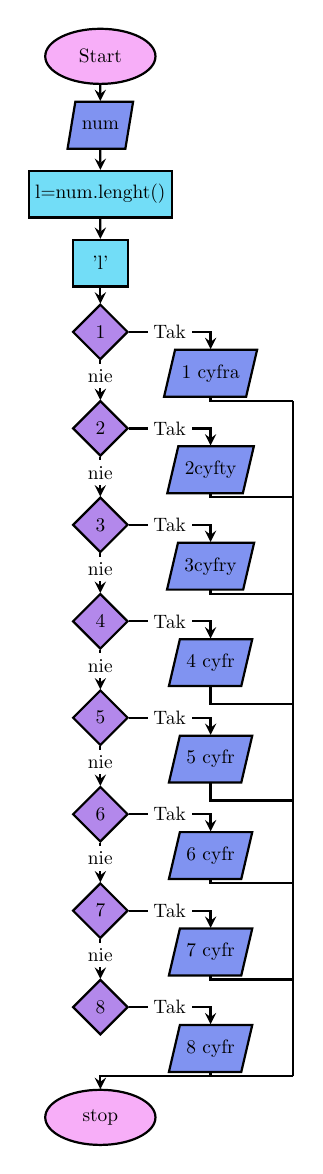
\begin{tikzpicture}[scale=0.7,transform shape]
		\node [style=startstop] (0) at (0, 0) {Start};
		\node [style=io] (1) at (0, -1.25) {num};
		\node [style=process] (3) at (0, -3.75) {'l'};
		\node [style=decision] (4) at (0, -5) {1};
		\node [style=decision] (5) at (0, -6.75) {2};
		\node [style=decision] (6) at (0, -8.5) {3};
		\node [style=decision] (7) at (0, -10.25) {4};
		\node [style=process] (8) at (0, -2.5) {l=num.lenght()};
		\node [style=decision] (9) at (0, -12) {5};
		\node [style=decision] (10) at (0, -13.75) {6};
		\node [style=decision] (11) at (0, -15.5) {7};
		\node [style=decision] (12) at (0, -17.25) {8};
		\node [style=io] (14) at (2, -5.75) {1 cyfra};
		\node [style=io] (15) at (2, -7.5) {2cyfty};
		\node [style=io] (16) at (2, -9.25) {3cyfry};
		\node [style=io] (17) at (2, -11) {4 cyfr};
		\node [style=io] (18) at (2, -12.75) {5 cyfr};
		\node [style=io] (19) at (2, -14.5) {6 cyfr};
		\node [style=io] (20) at (2, -16.25) {7 cyfr};
		\node [style=io] (21) at (2, -18) {8 cyfr};
		\node [style=startstop] (22) at (0, -19.25) {stop};
		\node [style=none] (23) at (3.5, -6.25) {};
		\node [style=none] (24) at (3.5, -8) {};
		\node [style=none] (25) at (3.5, -9.75) {};
		\node [style=none] (26) at (3.5, -11.75) {};
		\node [style=none] (27) at (3.5, -13.5) {};
		\node [style=none] (28) at (3.5, -15) {};
		\node [style=none] (29) at (3.5, -16.75) {};
		\node [style=none] (30) at (3.5, -18.5) {};

%\draw [arrow] (c3) -- (c4)node[pos=0.4,fill=white,inner sep=3]{nie};
%\draw [arrow] (c1) -| (p1)node[pos=0.25,fill=white,inner sep=3]{Tak};

		\draw [style=arrow] (0) to (1);
		\draw [style=arrow] (1) to (8);
		\draw [style=arrow] (8) to (3);
		\draw [style=arrow] (3) to (4);
		\draw [style=arrow] (4) -- (5)node[pos=0.4,fill=white,inner sep=3]{nie};
		\draw [style=arrow] (5) -- (6)node[pos=0.4,fill=white,inner sep=3]{nie};
		\draw [style=arrow] (6) -- (7)node[pos=0.4,fill=white,inner sep=3]{nie};
		\draw [style=arrow] (7) -- (9)node[pos=0.4,fill=white,inner sep=3]{nie};
		\draw [style=arrow] (9) -- (10)node[pos=0.4,fill=white,inner sep=3]{nie};
		\draw [style=arrow] (10) -- (11)node[pos=0.4,fill=white,inner sep=3]{nie};
		\draw [style=arrow] (11) -- (12)node[pos=0.4,fill=white,inner sep=3]{nie};
		\draw [style=arrow] (4) -| (14)node[pos=0.25,fill=white,inner sep=3]{Tak};
		\draw [style=arrow] (5) -| (15)node[pos=0.25,fill=white,inner sep=3]{Tak};
		\draw [style=arrow] (6) -| (16)node[pos=0.25,fill=white,inner sep=3]{Tak};
		\draw [style=arrow] (7) -| (17)node[pos=0.25,fill=white,inner sep=3]{Tak};
		\draw [style=arrow] (9) -| (18)node[pos=0.25,fill=white,inner sep=3]{Tak};
		\draw [style=arrow] (10) -| (19)node[pos=0.25,fill=white,inner sep=3]{Tak};
		\draw [style=arrow] (11) -| (20)node[pos=0.25,fill=white,inner sep=3]{Tak};
		\draw [style=arrow] (12) -| (21)node[pos=0.25,fill=white,inner sep=3]{Tak};
		\draw [style=con] (14) |- (23.center);
		\draw [style=con] (15) |- (24.center);
		\draw [style=con] (16) |- (25.center);
		\draw [style=con] (17) |- (26.center);
		\draw [style=con] (18) |- (27.center);
		\draw [style=con] (19) |- (28.center);
		\draw [style=con] (20) |- (29.center);
		\draw [style=con] (21) |- (30.center);
		\draw [style=con] (23.center) to (30.center);
		\draw [style=arrow] (30.center) -| (22);
\end{tikzpicture}
\caption{2.3 flowchart}
    \label{flow3}
\end{figure}   
        \end{minipage}  
\end{flushleft}
\subsection*{2.4}
\begin{minted}[framesep=1mm, baselinestretch=1.,linenos]{python}
print('ile jest liczb podzielnych przez c w <a;b>')
a=int(input('podaj a:'))
b=int(input('podaj b:'))
c=int(input('podaj c:'))
t=bool(a%c)
a=a+(c*t-a%c)
b=b-b%c
n=int((b-a)/c+1)
print(n,' liczb podzielnych przez ',c)
for i in range(0,n):print(a+c*i,',',end="")
\end{minted}
\subsection*{2.5}
\begin{minted}[framesep=1mm, baselinestretch=1.,linenos]{python}
print('program do liczenia śrdniej z n liczb')
n=int(input('podaj n:'))
sum=float(0)
for i in range(0,n):
    print('podaj ',i+1,':',end="")
    e=int(input())
    sum=sum+e
sum=round(sum/n,2)
print('średnia',n,'liczba jest równa: ',sum)
\end{minted}
\vspace{7.05cm}
\subsection*{2.6}
\begin{minted}[framesep=1mm, baselinestretch=1.,linenos]{cpp}
int n=0;cout<<"podaj n: ";cin>>n;
int l[3]= {0,0,0};int p=100;
for (int m=round(pow(75.8531-cos(-0.896604*n),\
cos(0.0903642*n-1.26534))-4.43137);m>0;p++)
{l[0]=floor(p/100);
l[1]=floor((p-l[0]*100)/10);
l[2]=p-(l[1]*10+l[0]*100);
if(l[0]+l[1]+l[2]==n){m--;cout<<p<<endl;}
}cout<<"liczbe możliwości: "<<i;
\end{minted}
\end{multicols}
\newpage

\begin{multicols}{2}
\begin{flushleft}
    \hspace{1cm}
    \begin{minipage}{3cm}
        \subsection*{2.7}
        \begin{tikzpicture}
	\begin{pgfonlayer}{nodelayer}
		\node [style=startstop] (0) at (0, 0.25) {Start};
		\node [style=process] (1) at (0, -1.25) {d='N'};
		\node [style=process] (2) at (0, -3) {2.6};
		\node [style=io] (3) at (0, -4.75) {toupper(d)};
		\node [style=decision] (4) at (0, -6.75) {d='T'|| d='N'};
		\node [style=decision] (5) at (1.5, -8.5) {d!='N'};
		\node [style=startstop] (6) at (0, -9.75) {Stop};
		\node [style=none] (7) at (0, -2) {};
		\node [style=none] (8) at (2.75, -2) {};
		\node [style=none] (9) at (-1.75, -3.75) {};
		\node [style=none] (10) at (0, -3.75) {};
	\end{pgfonlayer}
	\begin{pgfonlayer}{edgelayer}
		\draw [style=arrow] (0) to (1);
		\draw [style=arrow] (1) to (2);
		\draw [style=arrow] (2) to (3);
		\draw [style=arrow] (3) to (4);
		\draw [style=arrow] (4) to (5);
		\draw [style=arrow] (5) to (6);
		\draw (5) to (8.center);
		\draw (8.center) to (7.center);
		\draw (4) to (9.center);
		\draw (9.center) to (10.center);
	\end{pgfonlayer}
\end{tikzpicture}
    

        \subsection*{2.8}
        \renewcommand{\thefigure}{8}
\begin{figure}[H]
    \centering 
    %text width=1cm
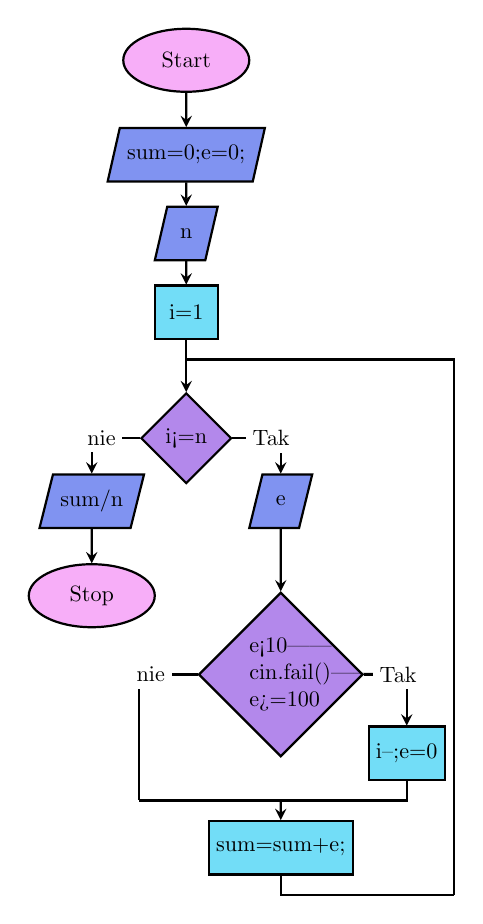
\begin{tikzpicture}[scale=0.8,transform shape]
		\node [style=startstop] (0) at (0, 0) {Start};
		\node [style=io] (1) at (0, -1.5) {sum=0;e=0;};
		\node [style=io] (2) at (0, -2.75) {n};
		\node [style=process] (3) at (0, -4) {i=1};
		\node [style=decision] (4) at (0, -6) {i<=n};
		\node [style=io] (5) at (1.5, -7) {e};
		\node [style=decision,text width=1cm] (6) at (1.5, -9.75) {e<10|| cin.fail()||  e>=100};
		\node [style=process] (7) at (3.5, -11) {i--;e=0};
		\node [style=process] (8) at (1.5, -12.5) {sum=sum+e;};
		\node [style=none] (9) at (1.5, -11.75) {};
		\node [style=none] (10) at (-0.75, -11.75) {};
		\node [style=none] (11) at (4.25, -13.25) {};
		\node [style=none] (12) at (0, -4.75) {};
		\node [style=io] (13) at (-1.5, -7) {sum/n};
		\node [style=startstop] (14) at (-1.5, -8.5) {Stop};

        % node[pos=0.4,fill=white,inner sep=3]{nie};
		% node[pos=0.25,fill=white,inner sep=3]{Tak};
        
		\draw [style=arrow] (2) to (3);
		\draw [style=arrow] (3) to (4);
		\draw [style=arrow] (4) -| (5)node[pos=0.4,fill=white,inner sep=3]{Tak};
		\draw [style=arrow] (5) to (6);
		\draw [style=arrow] (6) -| (7)node[pos=0.4,fill=white,inner sep=3]{Tak};
		\draw [style=con] (7) |- (9.center);
		\draw [style=con] (6) -| (10.center)node[pos=0.4,fill=white,inner sep=3]{nie};
		\draw [style=con] (10.center) to (9.center);
		\draw [style=arrow] (9.center) to (8);
		\draw [style=con] (8) |- (11.center);
		\draw [style=con] (11.center) |- (12.center);
		\draw [style=arrow] (0) to (1);
		\draw [style=arrow] (1) to (2);
		\draw [style=arrow] (4) -| (13)node[pos=0.4,fill=white,inner sep=3]{nie};
		\draw [style=arrow] (13) to (14);

\end{tikzpicture}
\caption{2.8 flowchart}
    \label{flow8}
\end{figure}
        
        \subsection*{2.9}
        \renewcommand{\thefigure}{9}
\begin{figure}[H]
    \centering 
    %text width=1cm
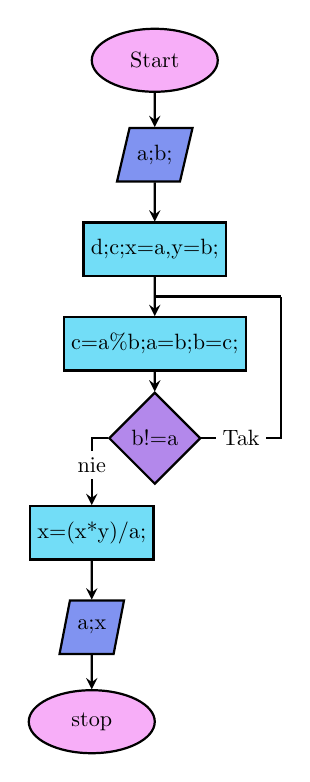
\begin{tikzpicture}[scale=0.8,transform shape]
        \node [style=startstop] (0) at (0, 0) {Start};
		\node [style=io] (1) at (0, -1.5) {a;b;};
		\node [style=process] (2) at (0, -3) {d;c;x=a,y=b;};
		\node [style=process] (3) at (0, -4.5) {c=a\%b;a=b;b=c;};
		\node [style=decision] (4) at (0, -6) {b!=a};
		\node [style=none] (5) at (2, -3.75) {};
		\node [style=none] (6) at (0, -3.75) {};
		\node [style=process] (7) at (-1, -7.5) {x=(x*y)/a;};
		\node [style=io] (8) at (-1, -9) {a;x};
		\node [style=startstop] (9) at (-1, -10.5) {stop};

        % node[pos=0.4,fill=white,inner sep=3]{nie};
		% node[pos=0.25,fill=white,inner sep=3]{Tak};

		\draw [style=arrow] (0) to (1);
		\draw [style=arrow] (1) to (2);
		\draw [style=arrow] (2) to (3);
		\draw [style=arrow] (3) to (4);
		\draw [style=arrow] (8) to (9);
		\draw [style=con] (4) -| (5.center)node[pos=0.25,fill=white,inner sep=3]{Tak};
		\draw [style=con] (5.center) to (6.center);
		\draw [style=arrow] (4) -| (7)node[pos=0.7,fill=white,inner sep=3]{nie};
		\draw [style=arrow] (7) to (8);
\end{tikzpicture}
\caption{2.9 flowchart}
    \label{flow9}
\end{figure}
 
        \end{minipage}  
\end{flushleft}
\begin{minipage}{3cm}
\vspace{10cm}
\subsection*{2.10}
\begin{minted}[framesep=1mm, baselinestretch=1.,linenos]{cpp}
int a[2]={0,16};
string c[2]={"min","max"};
int i;int x;int y;int l=4;
cout<<"program tabliczka mno�enie od do.\n\
Program przymuje wartości <-15;15>"<<endl;  
while(i<2){
cout<<"podaj "<<c[i]<<": ";
cin.clear();cin.sync();
a[i]=0;cin>>a[i];
if(cin.fail()||abs(a[i])>15||a[0]>a[1])
{cout<<endl<<"podana wartość jest nie poprawna"<<endl;
i--;}i++;}system("cls");y=a[0];
while (y<=a[1])
{
    x=a[0];cout<<y;gotoxy(3,y-a[0]+2);
    cout<<"|";
    while (x<=a[1]){
        gotoxy((x-a[0]+1)*l,y-a[0]+2);
        cout<<y*x;
        x++;}
    cout<<endl;y++;
}
\end{minted}
\end{minipage}
\end{multicols}
\newpage
\begin{multicols}{2}
\begin{flushleft}
    \hspace{1cm}
    \begin{minipage}{3cm}
        \subsection*{2.11}
        \begin{minted}[framesep=1mm, baselinestretch=1.,linenos]{cpp}
int i;int a;int min=100;
cout<<"program do szukania minimalne liczby\
z ciągu liczb dwu cyfrowych"<<endl;  
cout<<"aby zakończyć podawanie ciągu\
podaj liczbę 0"<<endl;  
while(a!=0)
{  
i++;cin.clear();cin.sync();
cout<<"podaj "<<i<<":";
a=0;cin>>a;        
if(a==0){break;}
else if(cin.fail()||abs(a)<10||abs(a)>99)
{cout<<"podana wartość jest nie poprawna"\
<<endl;i--;}
else{if(a<min){min=a;}}
}
cout<<"minimalną liczbą z ciągu:"<<endl;
if(min==100)
{cout<<"najmniejsza liczba ci¹gu nale¿y\
do zbioru pustego"<<endl;}
else{cout<<endl<<"jest: "<<min<<endl;}
\end{minted}    

        \subsection*{2.12}
        \begin{minted}[framesep=1mm, baselinestretch=1.,linenos]{cpp}
cout<<"program do nwd i nww"<<endl;  
int i;
char l='a';
int g[2]={0,0};      
while(i<2){
cout<<"podaj "<<l<<": ";
cin.clear();cin.sync();
g[i]=0;cin>>g[i];
if(cin.fail())
{cout<<endl<<"podana wartość jest nie poprawna"\
<<endl;i--;l--;}
i++;l++;}	
int a=abs(g[0]);int x=a;
int b=abs(g[1]);int y=b;     
while(a!=b)
{
	if(a>b){a=a-b;}
	else{b=b-a;}
}
x=(x*y)/a;
cout<<"nwd:"<<a<<" nww:"<<x<<endl;
\end{minted}
        
        \subsection*{2.13}
        \begin{minted}[framesep=1mm, baselinestretch=1.,linenos]{cpp}
cout<<"program liczenia silni z n"<<endl;   
int i;int n;long long s;
i=1;n=1;s=1;
cout<<"podaj n:";
cin.clear();cin.sync();cin>>n;
while(i<=n){s=s*i;i++;}
cout<<"silna z n jest równa:"<<s<<endl;
\end{minted}
 
        \end{minipage}  
\end{flushleft}
\begin{minipage}{3cm}
\vspace{10.81cm}
\subsection*{2.14}
\begin{minted}[framesep=1mm, baselinestretch=1.,linenos]{cpp}
cout<<endl<<"program do liczenie n liczby fibonacciego"<<endl;  
cout<<"\npodaj n:";
int n = 0;
cin>>n;
if(cin.fail()){r=false;cout<<endl<<"podana wartość jest nie poprawna"<<endl;}
int i = 0;
double a=0;double b=1;double c=0;
while (n>i)
{c=a+b;a=b;b=c;i++;}
cout<<n<<" liczba ciagu fibonacciego jest rowna:"<<a<<endl;
\end{minted}
\end{minipage}
\end{multicols}
\newpage
\begin{multicols}{2}
\hspace{0.4cm}
\begin{minipage}{3cm}
\subsection*{2.15}
\begin{minted}[framesep=1mm, baselinestretch=1.,linenos]{python}
import math
print('sprawdzanie czy liczba jest pierwsza')
i=int(2)
n=int(1)
odp='tak'
while True:
    try:
        n=int(input('podaj a liczbe:'))
        break   
    except ValueError:print('zła wartość')

while i<=math.sqrt(n):
    if n%i==0:
        odp='nie'
        break
    i=i+1
print(odp)
\end{minted}  
\end{minipage}

\subsection*{2.16}
\begin{tikzpicture}
	\begin{pgfonlayer}{nodelayer}
		\node [style=startstop] (0) at (0, 0) {Start};
		\node [style=process] (1) at (0, -1.5) {n=1;s=0};
		\node [style=io] (2) at (0, -3) {n};
		\node [style=decision] (3) at (0, -5) {n==0};
		\node [style=io] (4) at (1.25, -6) {s};
		\node [style=startstop] (5) at (1.25, -7.5) {Stop};
		\node [style=process] (6) at (-1.5, -6.25) {s=s+n\%10; n=n/10};
		\node [style=none] (7) at (-2.75, -7.5) {};
		\node [style=none] (8) at (0, -3.75) {};
	\end{pgfonlayer}
	\begin{pgfonlayer}{edgelayer}
		\draw [style=arrow] (0) to (1);
		\draw [style=arrow] (1) to (2);
		\draw [style=arrow] (2) to (3);
		\draw [style=arrow] (3) to (4);
		\draw [style=arrow] (4) to (5);
		\draw [style=arrow] (3) to (6);
		\draw [style=con] (6) to (7.center);
		\draw [style=con] (7.center) to (8.center);
	\end{pgfonlayer}
\end{tikzpicture}
   
\end{multicols}




%--------------Programy użyte----------
\section{Programy użyte do wykonoania zadań}  
\LaTeX, tikzit, firefox, overleaf, dev c++, c++, python, visual studio code, notepad++, git, github, Sumatra PDF, Total comander  
\section{Wnioski i uwagi} 
\begin{center}
 \large{Zadanie mi się bardzo podobało i nie mam żadnych uwag.}   
\end{center}
 
\end{document}
